\chapter{Marco Te\'orico}
El presente capítulo permite conocer los conceptos básicos necesarios para el entendimiento del desarrollo acorde al proyecto propuesto. El campo de los biosensores se integra de conceptos elementales de electrónica, química, ciencia de los materiales y biología. La electrónica impresa funcional y las impresoras a chorro de tinta precisan de aclaraciones teóricas acordes al proyecto que se desarrollará. Se analizarán principios fundamentales de biosensores, las técnicas de electrónica impresa funcional, la impresión mediante chorro de tinta, los materiales a utilizar y las caracterizaciones a realizar.

\section{Sensores, transductores y biosensores}
Un \textbf{sensor} es un dispositivo capaz de transformar magnitudes físicas o químicas, llamadas variables de instrumentación, en magnitudes eléctricas a través de un transductor. Estos dispositivos pueden ser caracterizados por diferentes propiedades como el rango de medida, la precisión, la linealidad, la repetitividad, entre otros. Las variables de instrumentación pueden ser magnitudes como temperatura, presión, humedad, pH, intensidad lumínica, distancia, aceleración, inclinación, desplazamiento, fuerza, torsión, movimiento, etc. En un significado más extenso, es la ampliación de los sentidos para adquirir un conocimiento de cantidades fisicoquímicas que, por su naturaleza o tamaño, no pueden ser percibidas directamente por los sentidos \cite{PallasAreny}.

Un \textbf{transductor} transforma la variación de la propiedad del sensor en una salida de información detectable por un sistema electrónico. Puede poseer o no un acondicionador de señal dentro del mismo dispositivo, típicamente con alguna de las salidas de uso industrial: salida en tensión (V) o salida normalizada en corriente (4 a 20 mA)(Figura ~\ref{fig:Figura_concepto_sensor}).

\begin{figure}[H]
  \centering
    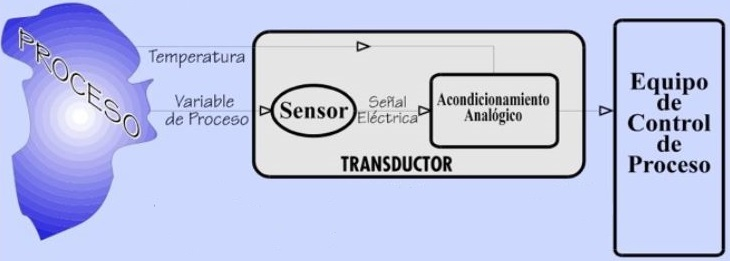
\includegraphics[width=0.8\textwidth]{Figuras/Figura_concepto_sensor}
  \caption{Diagrama sensor y transductor. Figura extraída de \cite{Hector1}.}
  \label{fig:Figura_concepto_sensor}
\end{figure}

Un \textbf{biosensor} se puede definir como un dispositivo que reconoce un determinado analito mediante un \textbf{biorreceptor} acoplado a un \textbf{transductor fisicoquímico} que convierte la señal biológica en una señal eléctrica (Figura ~\ref{fig:Figura_Biosensor}), siendo esta señal proporcional al grupo de compuestos que se quiere determinar cualitativa o cuantitativamente. Un analito es el componente de interés analítico de una muestra. En el caso de los biosensores, son ejemplos una molécula de proteína, una toxina, un péptido, una vitamina o un ion metálico. El biorreceptor puede ser una biomolécula simple o compleja (enzimas, anticuerpos, cadenas de ácidos nucleicos), o basado en células (tejidos, organismos) y puede ser tomado de la naturaleza o sintetizado en un laboratorio. El transductor puede ser del tipo resonante, óptico, térmico, transistor de efecto de campo FET (\textit{Field-Effect Transistor}), de ondas acústicas superficiales (\textit{Surface Acoustic Wave}), piezoeléctrico o electroquímico. Dentro de este último se pueden diferenciar los del tipo conductímetro, amperométrico, potenciométrico e impedométrico \cite{Eggins}.

\begin{figure}[H]
  \centering
    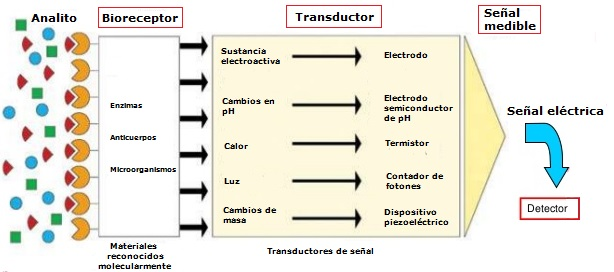
\includegraphics[width=0.8\textwidth]{Figuras/Figura_Biosensor}
  \caption{Diagrama de biosensor: biorreceptor, transductor y acondicionador de señal electrónico. Figura extraída de \cite{Lili1}.}
  \label{fig:Figura_Biosensor}
\end{figure}

Los transductores electroquímicos son los más utilizados en el desarrollo de biosensores enzimáticos. Esto se debe a que poseen una serie de ventajas, tales como:

$\bullet$ Las medidas electroquímicas pueden ser realizadas en volúmenes pequeños, incluso del orden de nanolitros, con relativa facilidad. Esto hace que tales dispositivos sean especialmente apropiados para monitorizar $``$\textit{in vivo}$"$.

$\bullet$ La señal eléctrica obtenida es la transducción directa de la velocidad de reacción química.

$\bullet$ Los límites de detección que se obtienen, normalmente entre 10\textsuperscript{-9} y 10\textsuperscript{-6} mol$\cdot$l\textsuperscript{-1}, son suficientes y adecuados para la detección de numerosos analitos de interés.

$\bullet$ La relativa simplicidad y el bajo costo de la instrumentación electroquímica permiten una fácil disponibilidad de estos dispositivos.


Sin duda alguna, en el contexto de los biosensores electroquímicos, los más prometedores en términos de sensibilidad, selectividad, tamaño, portabilidad y un mínimo volúmen de muestra (analito) necesaria, son los biosensores amperométricos, objeto de estudio del presente proyecto final integrador. Dichos sensores monitorizan corrientes faradaicas (transferencia directa de electrones vía una reacción de oxidación en un electrodo y una reacción de reducción en el otro) entre el sistema biológico y una celda electroquímica típica conformada por tres electrodos: un electrodo de trabajo \emph{(WE)}, uno de referencia \emph{(RE)} y un contra electrodo \emph{(CE)} (Figura ~\ref{fig:Figura_Definicion_Electrodo}). En el \emph{WE} ocurre la reacción electroquímica, para lo cual se le aplica un potencial variable respecto del electrodo de potencial fijo \emph{(RE)}. La corriente resultante de la reacción química circula entre el \emph{WE} y el \emph{CE}. La variación de potencial aplicado y la medición de corriente se controlan mediante un potenciostato.

\begin{figure}[H]
  \centering
    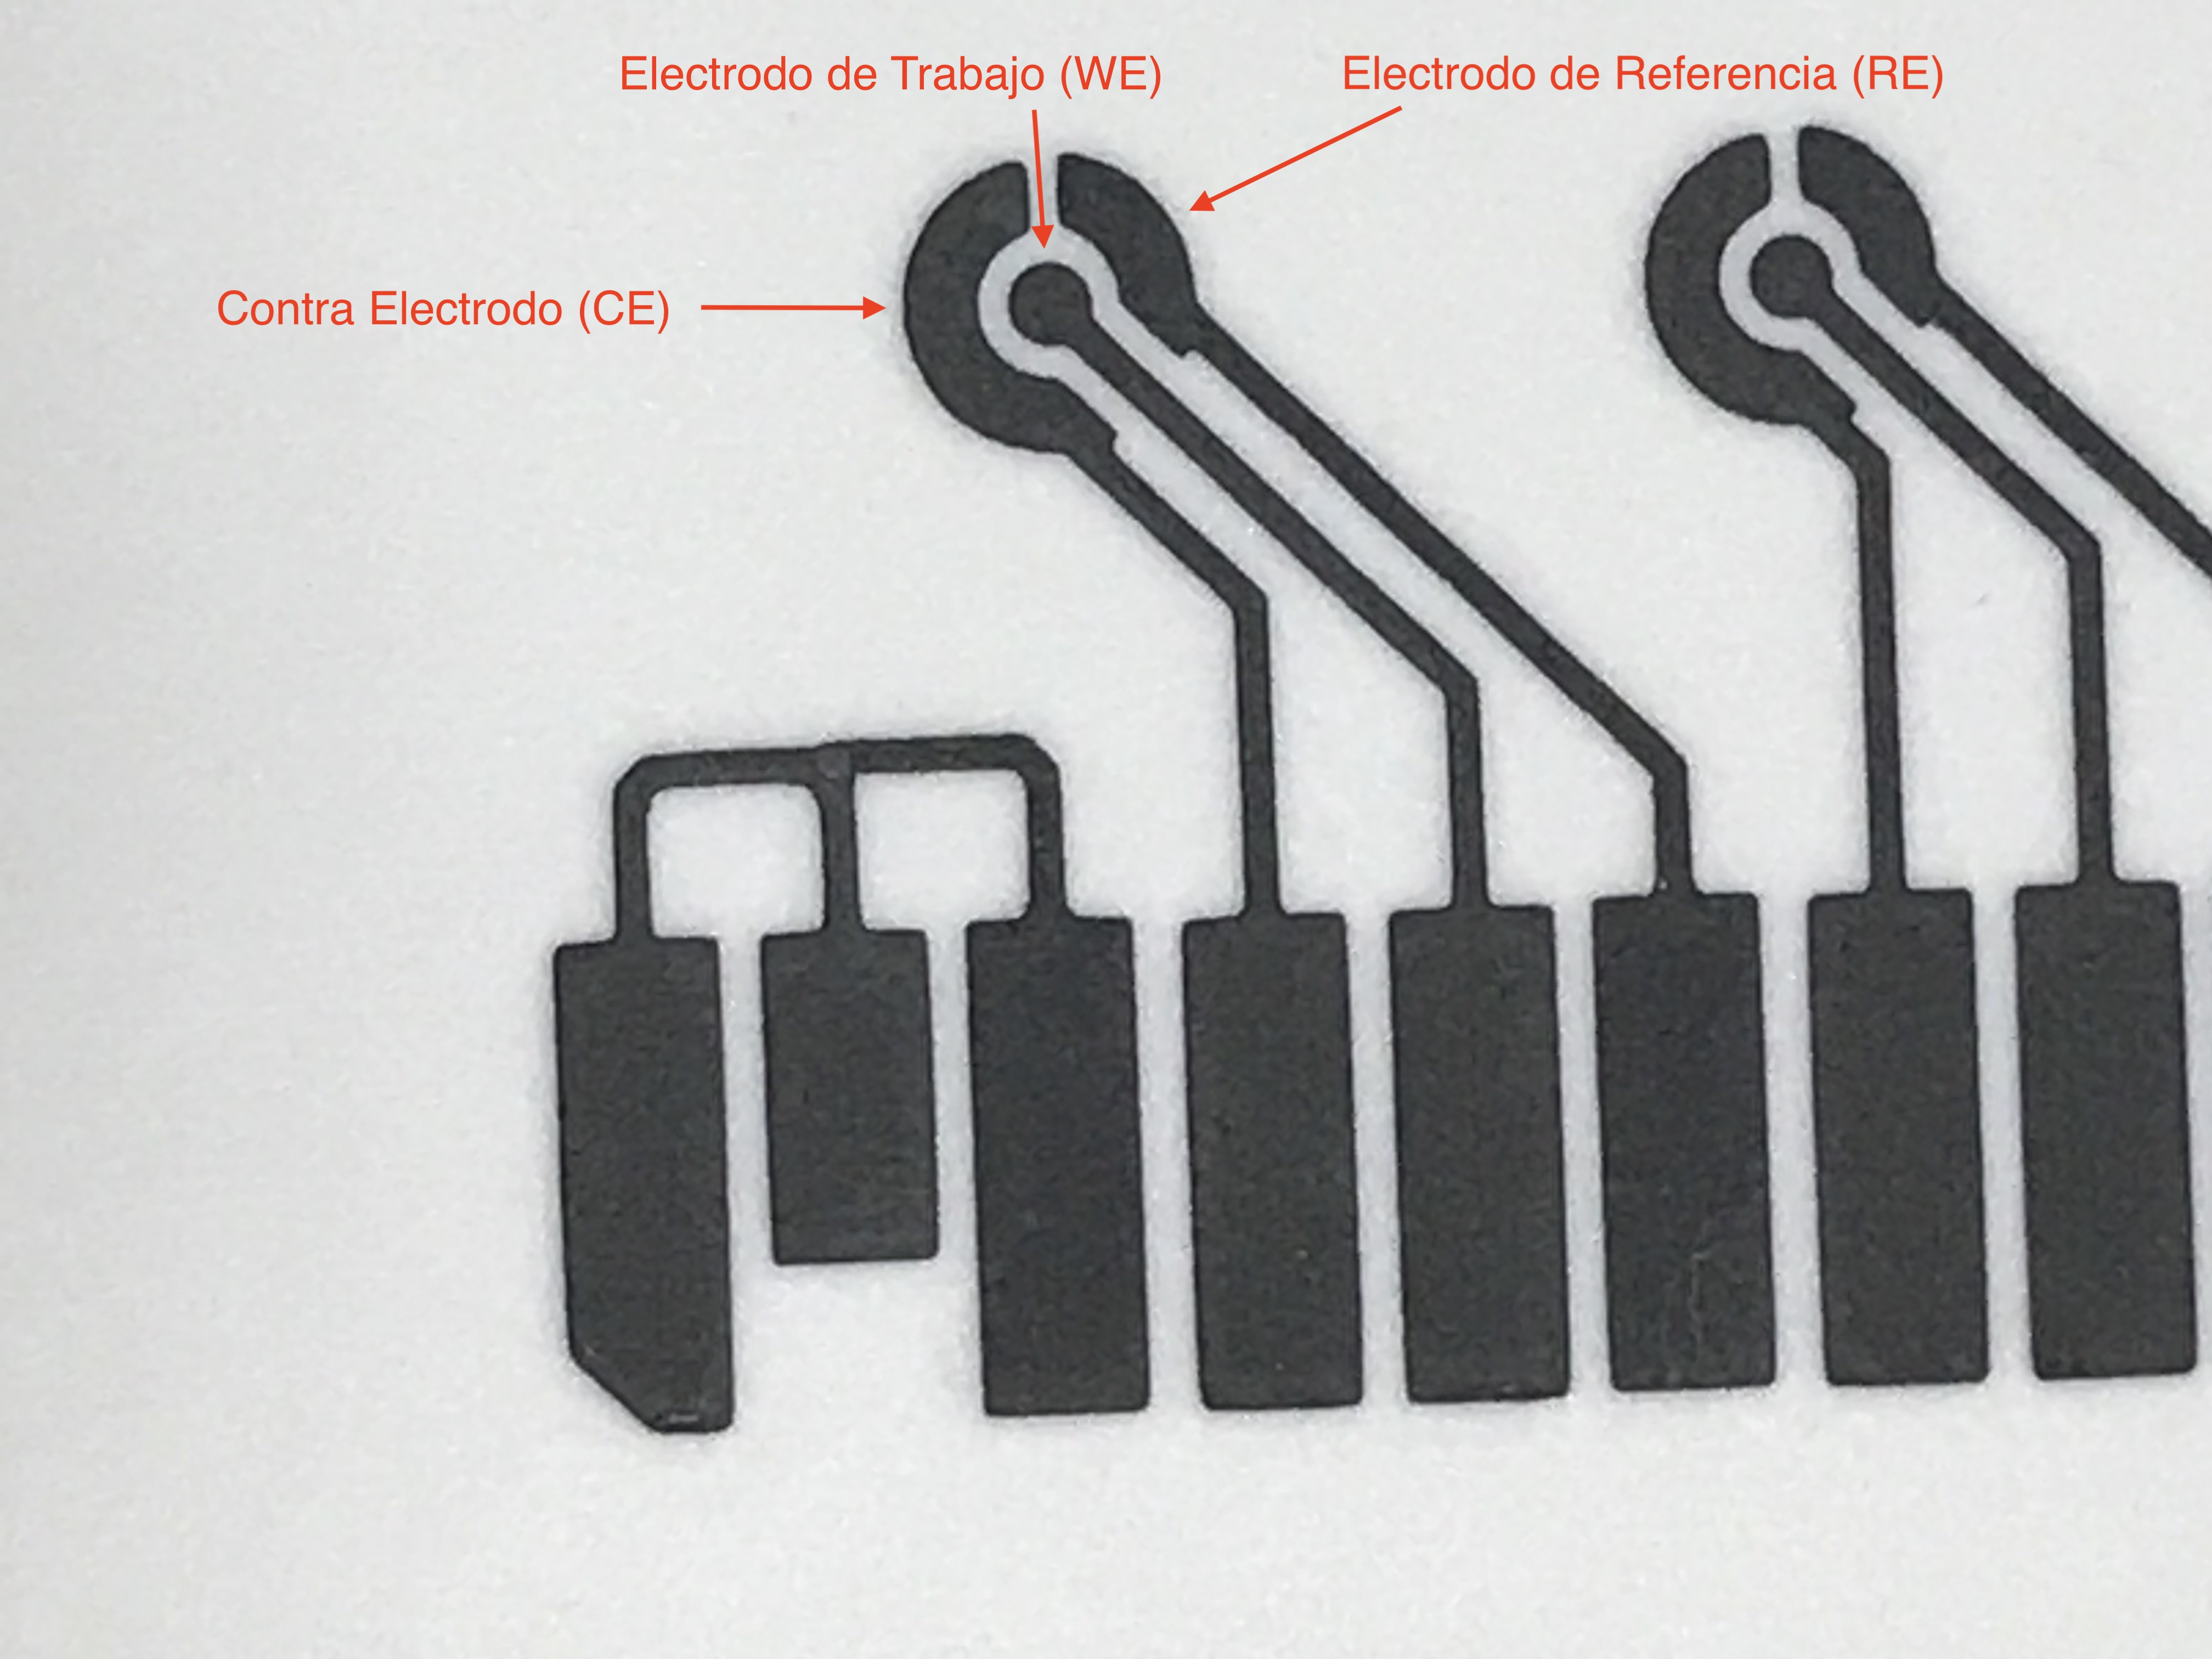
\includegraphics[width=0.5\textwidth]{Figuras/Figura_Definicion_Electrodo}
  \caption{Biosensor Electroquímico.}
  \label{fig:Figura_Definicion_Electrodo}
\end{figure}

Un potenciostato (Figura ~\ref{fig:Figura_potenciostato}) es un dispositivo electrónico utilizado para controlar una celda de tres electrodos y poder realizar la mayoría de los experimentos electroanalíticos. Su función es aplicar un potencial variable sobre el \emph{WE} respecto del potencial fijo aplicado sobre el \emph{RE} y medir la corriente resultante que circula entre el \emph{WE} (donde ocurre la reacción electroquímica) y el \emph{CE}.

\begin{figure}[H]
  \centering
    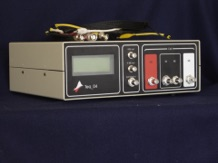
\includegraphics[width=0.5\textwidth]{Figuras/Figura_potenciostato}
  \caption{Potenciostato utilizado para la caracterización electroquímica.}
  \label{fig:Figura_potenciostato}
\end{figure}

\section{Electr\'onica Impresa Funcional}
Aprovechando los avances tecnológicos en micro y nano electrónica, se decidió implementar los biosensores utilizando técnicas de impresión, buscando de esta manera contar con cartuchos de arreglos de sensores descartables, de simple fabricación y alta escala de producción. Dichos biosensores se pueden imprimir sobre sustratos cerámicos (Al\textsubscript{2}O\textsubscript{3}), acrílicos o PMMA (Polímero de Metil Metacrilato), o sobre material flexible tipo PET (PoliEtileno Tereftalato), Valox, etc., utilizando diferentes técnicas, tales como impresión serigráfica ($``$\textit{Screen Printing}$"$) o impresión a chorro de tinta ($``$\textit{Inkjet}$"$).

La impresión serigráfica, propia de la tecnología de película gruesa, permite fabricar circuitos electrónicos y sensores que se obtienen al depositar capas de tintas (típicamente resistivas, conductoras y dieléctricas), por medio de una espátula de goma que se desplaza transversalmente a través de una malla o máscara, con un patrón dado, sobre un sustrato aislado, generalmente cerámica. La espátula fuerza la tinta a atravesar las aberturas de la malla que es de acero inoxidable. Posteriormente se sinterizan a temperaturas pico de 850ºC para remover los solventes de las tintas, fijar las características eléctricas de las tintas y adherir las capas al sustrato (Figura ~\ref{fig:Figura_serigrafia}).

\begin{figure}[H]
  \centering
    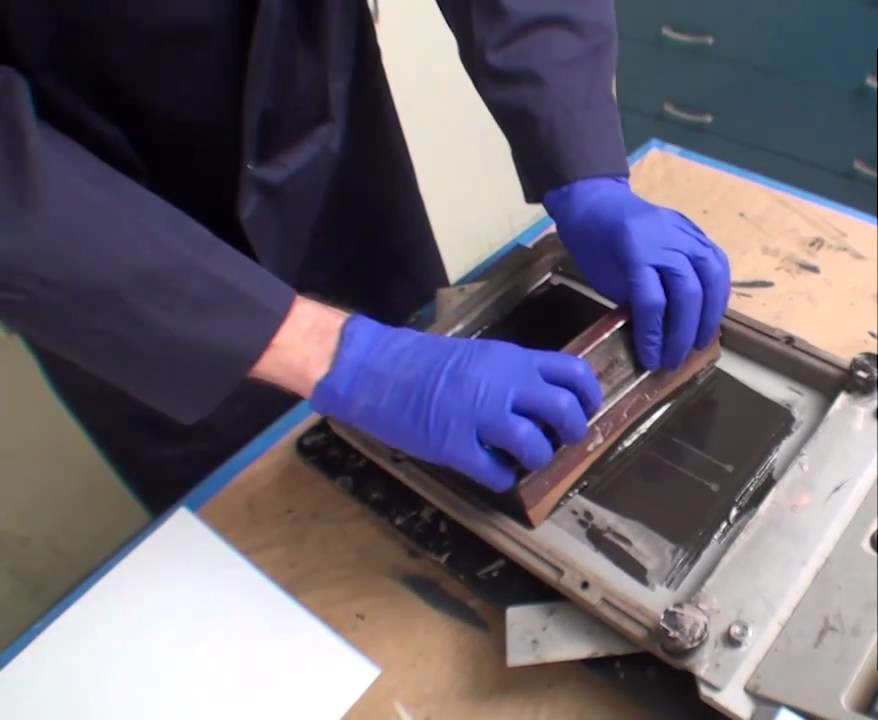
\includegraphics[width=0.5\textwidth]{Figuras/Figura_serigrafia}
  \caption{Impresión serigráfica manual.}
  \label{fig:Figura_serigrafia}
\end{figure}


La impresión a chorro de tinta utiliza cabezales piezoeléctricos para depositar gotas de tinta según coordenadas controladas por software. Las tintas pueden ser conductoras, semiconductoras o dieléctricas (Figura ~\ref{fig:Figura_inkjet_dimatix}).

\begin{figure}[H]
  \centering
    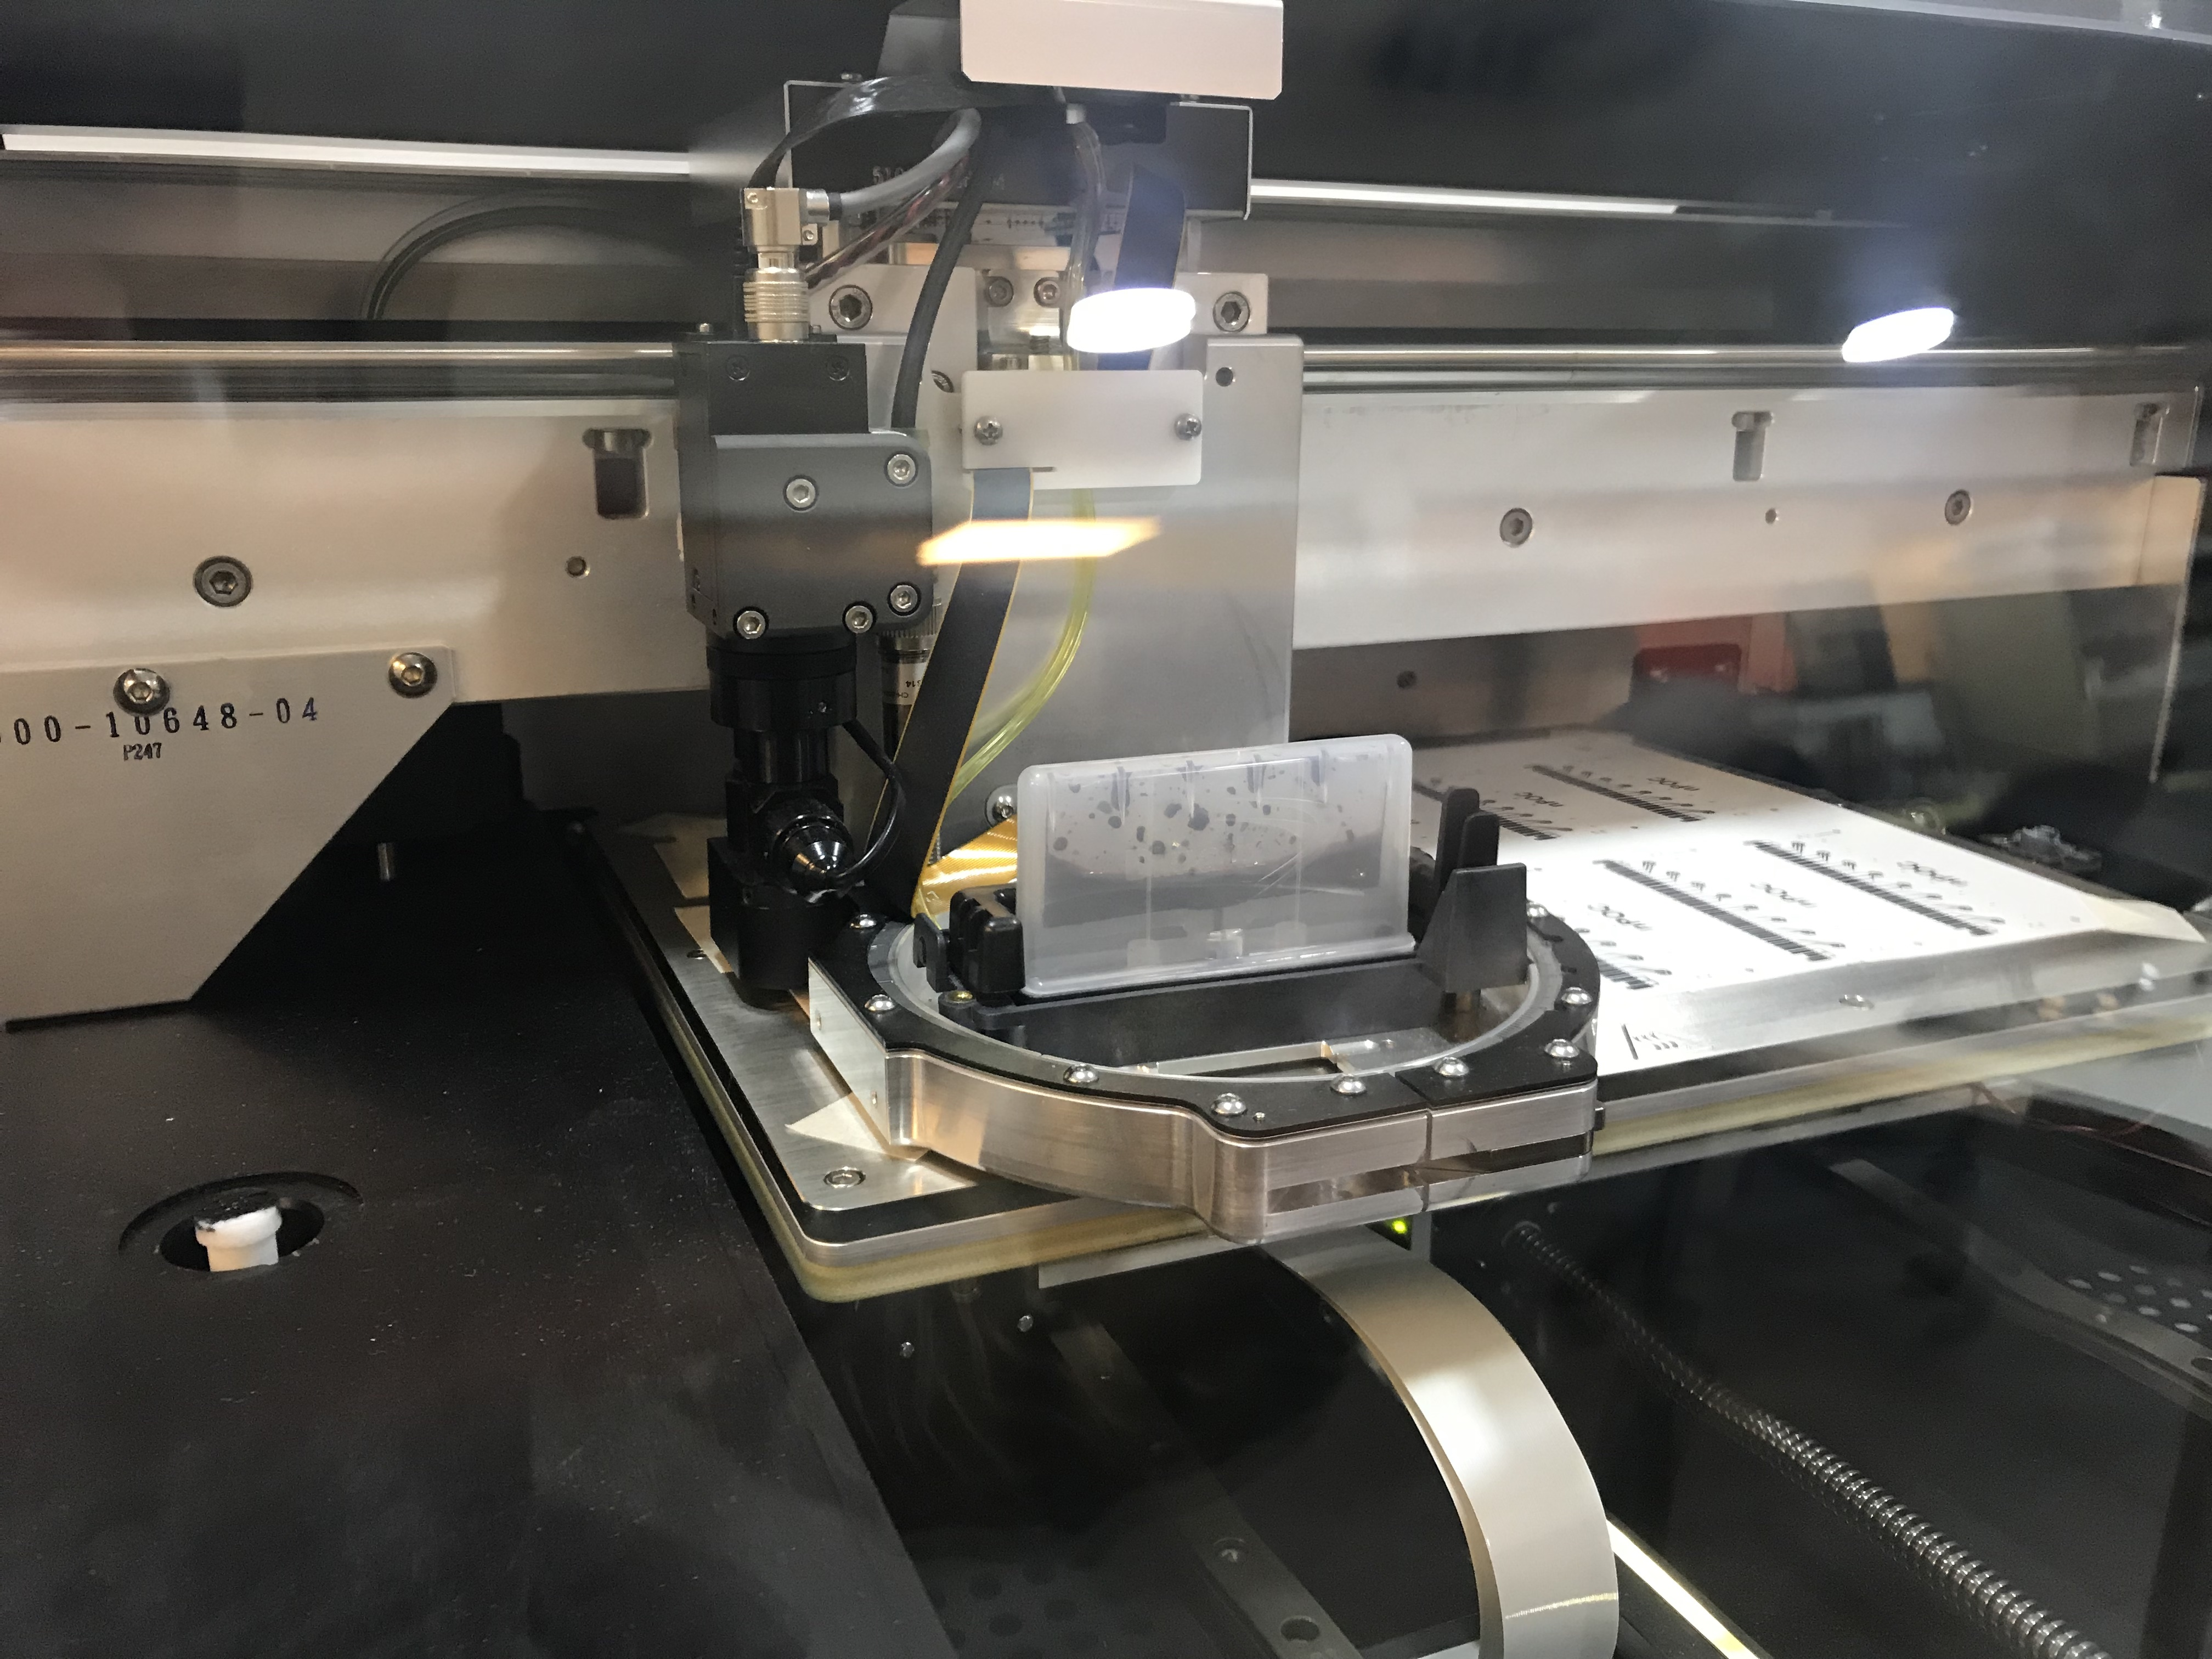
\includegraphics[width=0.5\textwidth]{Figuras/Figura_inkjet_dimatix}
  \caption{Impresión a chorro de tinta.}
  \label{fig:Figura_inkjet_dimatix}
\end{figure}


En esta tesis se implementa un biosensor electroquímico sobre sustrato flexible mediante una impresora \textit{Inkjet} y se utiliza el método amperométrico para caracterizarlo. La versatilidad, facilidad de uso y el tipo de fabricación innovador son algunas de las razones más destacables por las que se decidió realizar el presente proyecto en una impresora de chorro de tinta.

\subsection{Impresora tipo \textit{Inkjet}}
Como se mencionó la impresora tipo \textit{Inkjet} utiliza un cabezal piezoeléctrico para la deposición de tintas (Figura ~\ref{fig:Figura_Piezoelectrico}). Dicho cabezal contiene un reservorio con un cristal que, al aplicársele un potencial, se mueve generando una fuerza mecánica en el tanque, lo que provoca la eyección de una gota de tinta.

\begin{figure}[H]
  \centering
    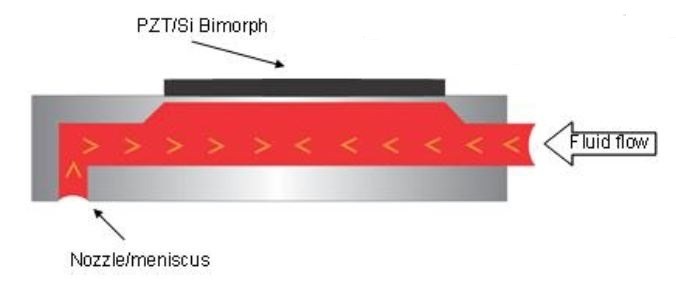
\includegraphics[width=0.5\textwidth]{Figuras/Figura_Piezoelectrico}
  \caption{Esquema de cabezal Piezoeléctrico.}
  \label{fig:Figura_Piezoelectrico}
\end{figure}

Para ello, se debe aplicar una forma de onda especificada por el fabricante (Figura ~\ref{fig:Figura_Waveform_Dimatix}), aunque esta debe ser modificada para cada tipo de tinta. 

\begin{figure}[H]
  \centering
    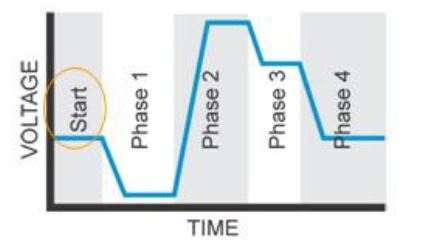
\includegraphics[width=0.5\textwidth]{Figuras/Figura_Waveform_Dimatix}
  \caption{Forma de onda especificada para cabezal de impresión piezoeléctrico.}
  \label{fig:Figura_Waveform_Dimatix}
\end{figure}

En la etapa denominada $``$\textit{Start}$"$ o también identificada como $``$\textit{Standby}$"$, el piezoeléctrico está levemente deflectado generando un menisco de tinta, evitando la caída involuntaria de tinta. En la etapa $``$\textit{Phase 1}$"$ se disminuye el potencial y el piezoeléctrico se mueve hacia arriba, permitiendo el llenado del reservorio. En la etapa $``$\textit{Phase 2}$"$ se incrementa la tensión, iniciando la formación de la gota. Una vez formada la gota, en la etapa $``$\textit{Phase 3}$"$ se vuelve a disminuir la tension, desprendiéndose la gota del cabezal. La etapa $``$\textit{Phase 4}$"$ es el retorno a la tensión de $``$\textit{Start}$"$ (Figura ~\ref{fig:Figura_etapas_eyector}).

\begin{figure}[H]
  \centering
    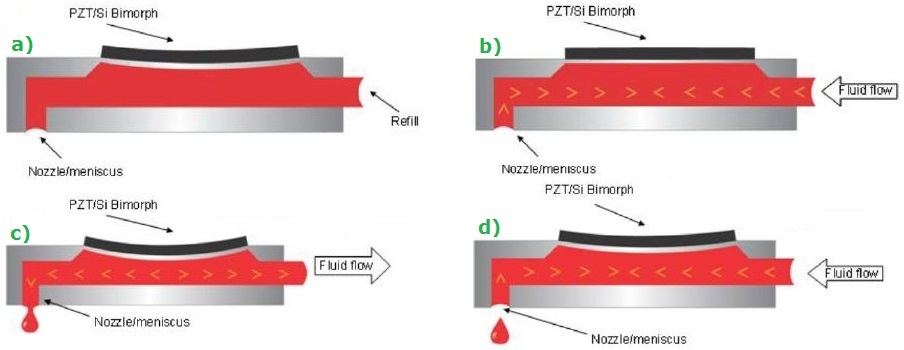
\includegraphics[width=0.8\textwidth]{Figuras/Figura_etapas_eyector}
  \caption{a) Etapa Start/Standby, b) Etapa 1, c) Etapa 2, d) Etapa 3 y vuelta a Standby.}
  \label{fig:Figura_etapas_eyector}
\end{figure}

Los parámetros modificables de esta forma de onda son el nivel de tensión (porcentaje relativo a la tensión seteada al eyector), velocidad de subida (\textit{Slew rate}) que especifica la pendiente de las rampas entre fases y la duración de cada segmento \cite{DimatixUM}.

El cabezal, responsable de eyectar la tinta es una pieza del tipo \textit{MEMS} (Sistemas-Micro-Electro-Mecánicos). Debido a esto son del tamaño convencional de una impresora de inyección térmica, pero de una tecnología superior (Figura ~\ref{fig:Figura_cabezal}). 

\begin{figure}[H]
  \centering
    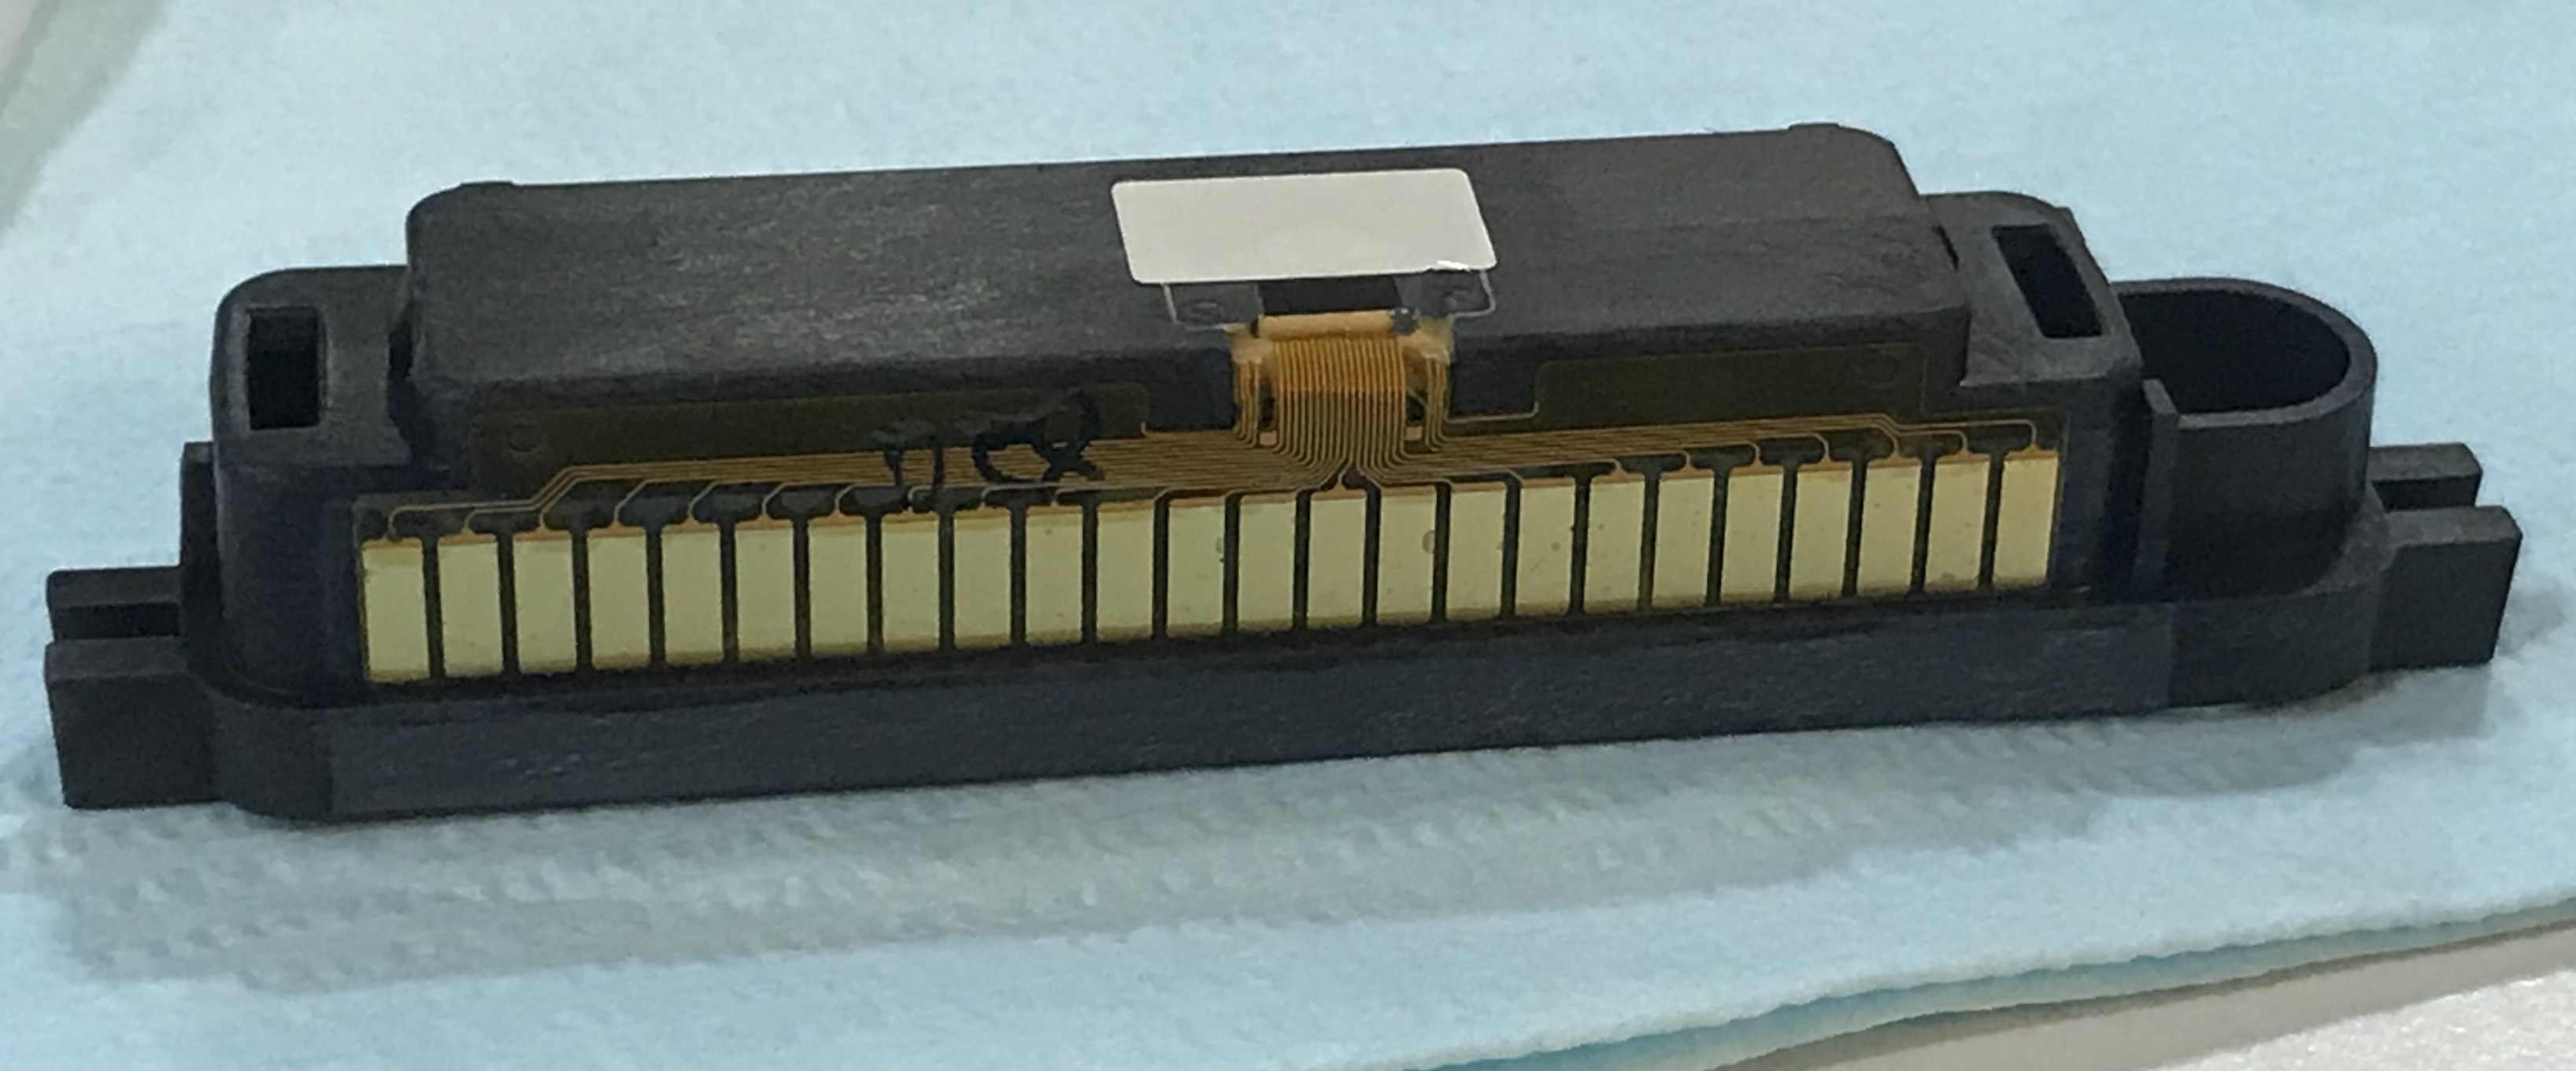
\includegraphics[width=0.5\textwidth]{Figuras/Figura_cabezal}
  \caption{Cabezal de impresora Fujifilm Dimatix DMP-2850.}
  \label{fig:Figura_cabezal}
\end{figure}

El correspondiente a la impresora Fujifilm Dimatix DMP2850 posee 16 eyectores, con los que se puede realizar distintas combinaciones, logrando diferentes espaciados entre gotas y por ende, distintos anchos de líneas. El cartucho completo consta del cabezal y un reservorio de 3 ml, que puede ser llenado con tintas de diferentes materiales (Figura ~\ref{fig:Figura_cartucho_completo}).

\begin{figure}[H]
  \centering
    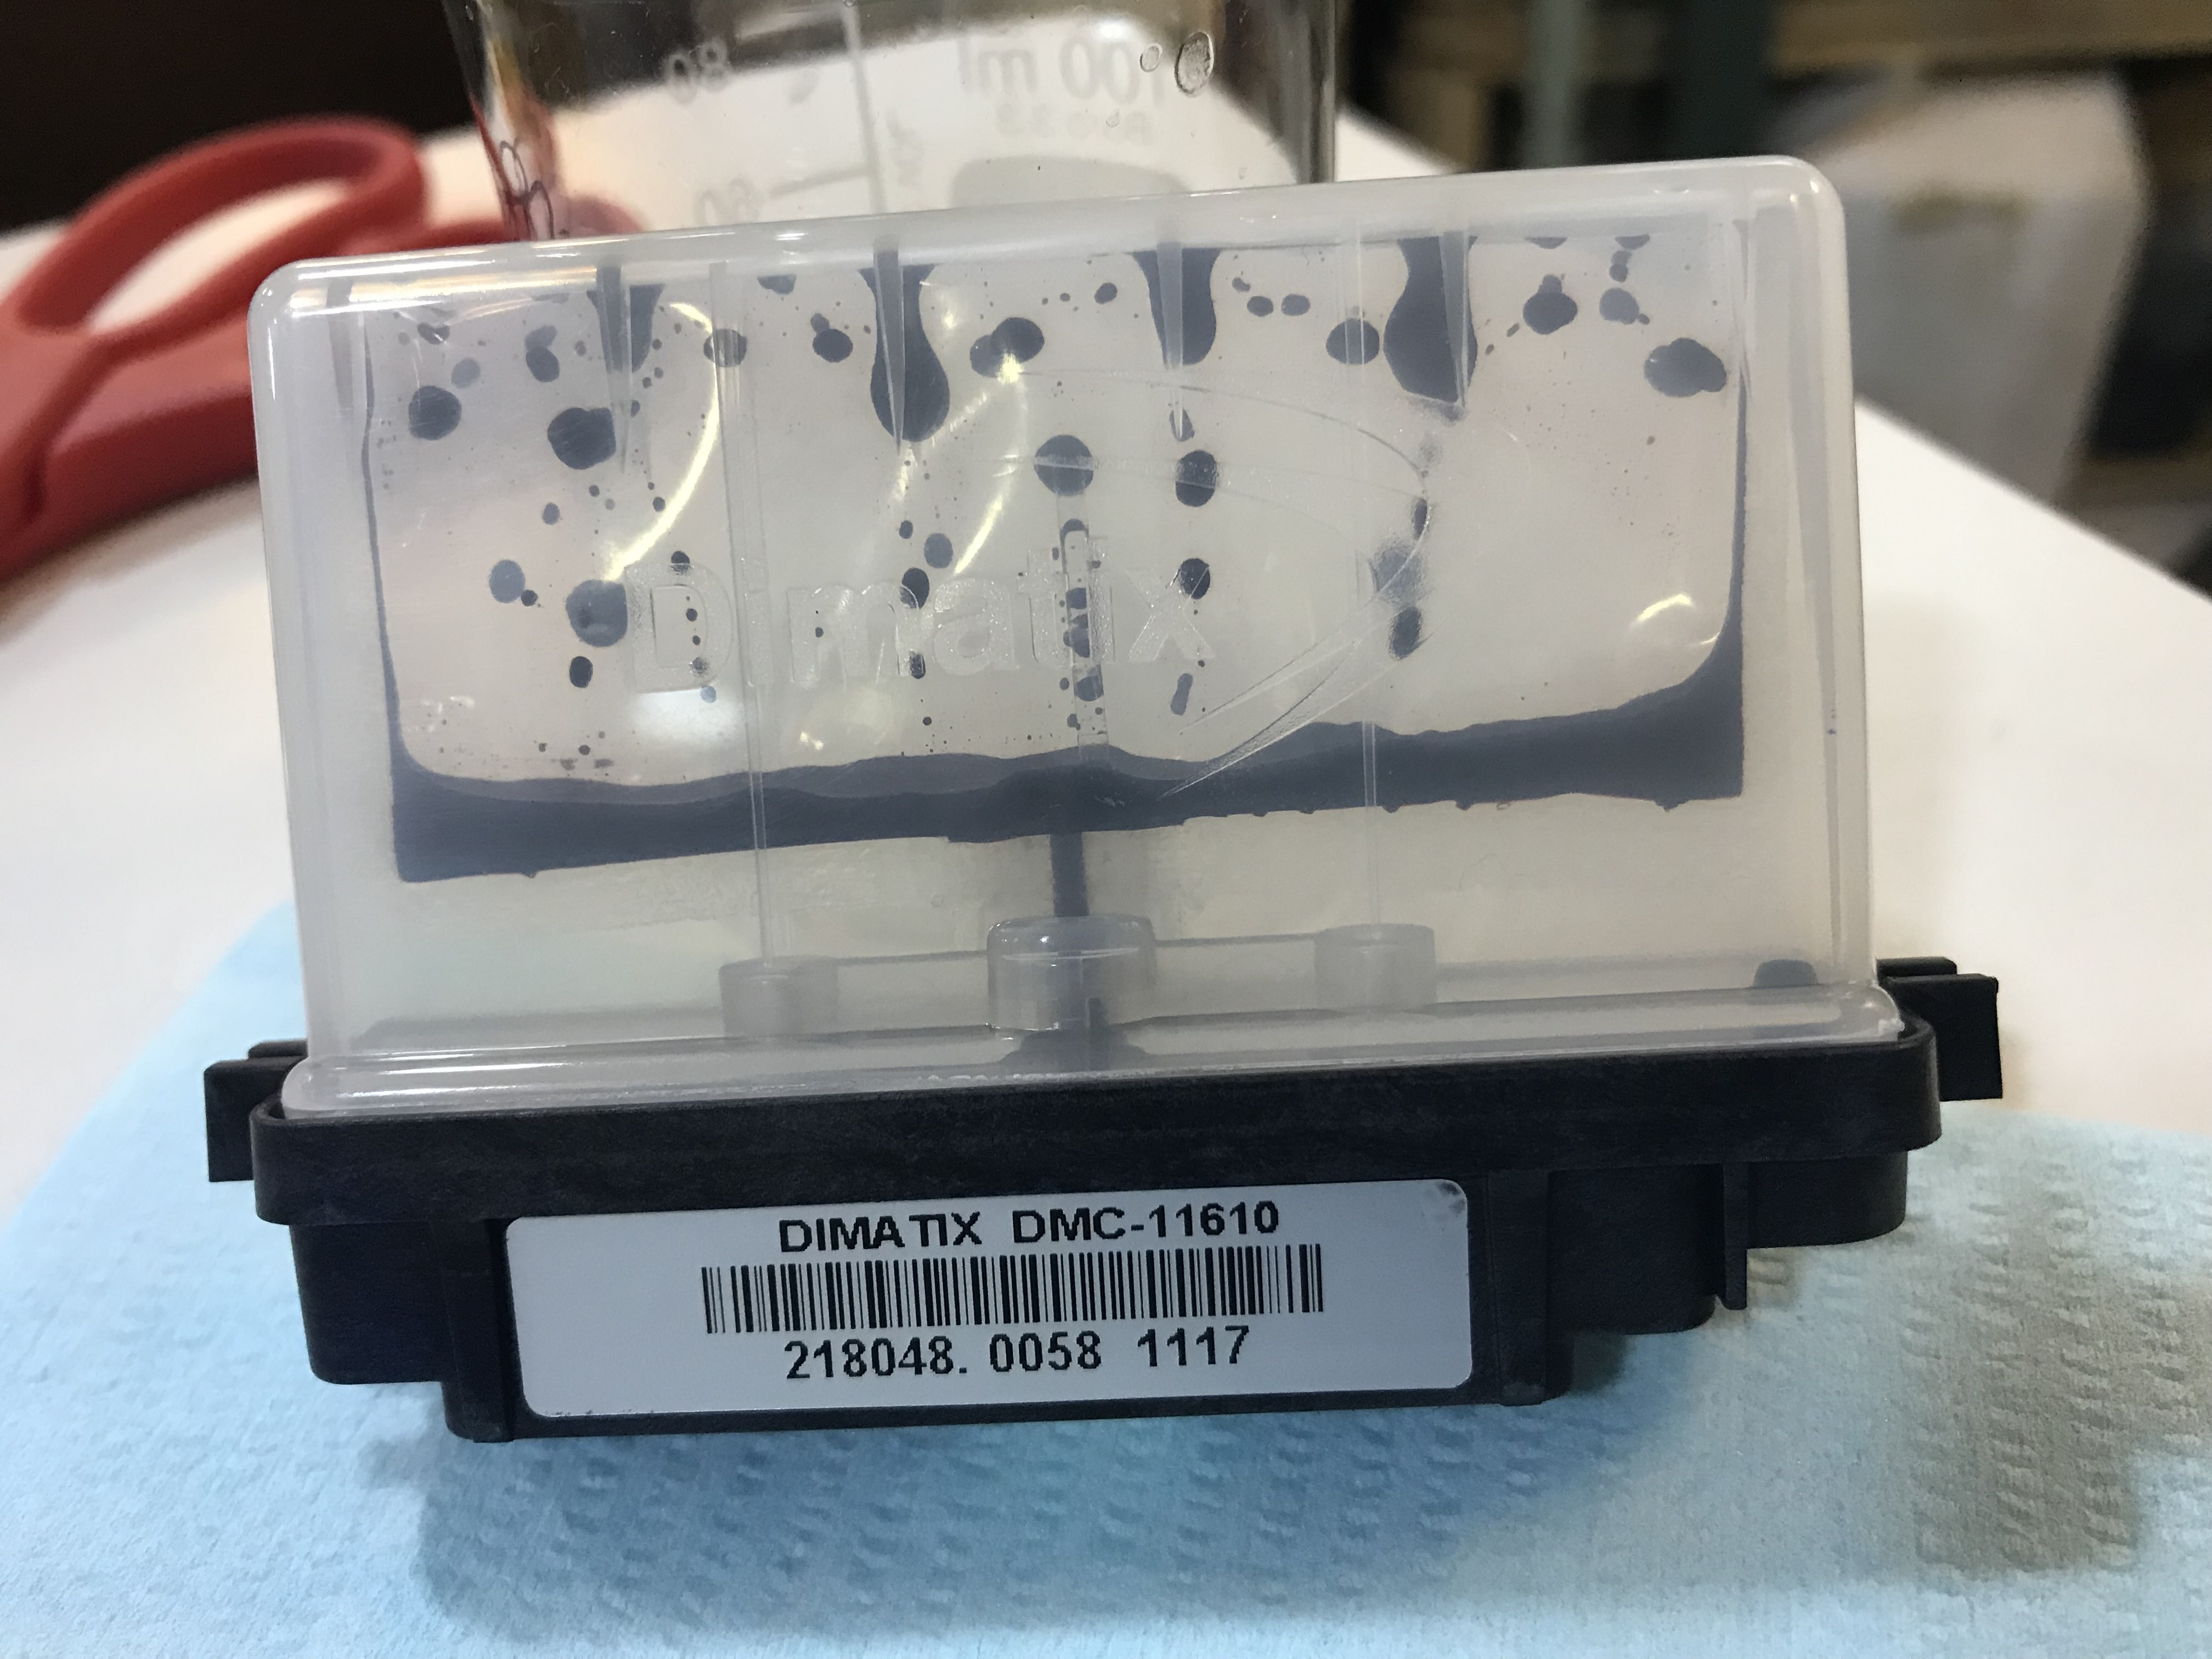
\includegraphics[width=0.5\textwidth]{Figuras/Figura_cartucho_completo}
  \caption{Cartucho de impresora Fujifilm Dimatix DMP-2850.}
  \label{fig:Figura_cartucho_completo}
\end{figure}

Como ejemplos, Fujifilm informa que puede imprimirse gráfica, electrónica, \textit{displays}, químicos, objetos ópticos, objetos fotovoltáicos, objetos mecánicos en 3D y elementos de la ciencia de la vida como cadenas de ADN.

\subsection{Tinta de nanopartículas de oro}
En este proyecto se utilizará una tinta con nanopartículas de oro, fabricada por \textit{C-INK Company} bajo el nombre comercial de \textit{Drycure Au-JB 1010B} \cite{DrycureAu}. Esta tinta contiene partículas nanométricas de oro (Au). Si bien no está comprobado el efecto de las mismas en el cuerpo humano, debe tenerse extrema precaución al manipularla. Por esto, el fabricante recomienda utilizarla en un ambiente con buena ventilación o sistema de extracción, utilizar protección respiratoria en caso de presentarse vapores. En todo momento deben usarse guantes, anteojos y ropa de trabajo, sobretodo al momento de manipular la tinta.

Dentro de su composición se tiene, dado como porcentaje en peso, 9-11 \% de Oro, 36-40 \% de agua, 48-52 \% de Glycerol, 0.1-1.0 \% de Alcohol, 0.1-0.5 \% de \textit{Acetylene glycol} y 0.1-2.0 \% de resina Polyester.

Como caracteristicas físicas y químicas, se indica que la tinta es liquida, es una solución miscible, tiene una densidad de 1.10 a 1.20 g/ml y una viscosidad de 9 a 11 mPa$\cdot$s.

Dado que la tinta está formulada a base de agua, debe mantenerse a bajas temperaturas y sellada hermeticamente para evitar la evaporación del solvente o la excesiva humedad, que pueden provocar cambios en sus características (Figura ~\ref{fig:Figura_tinta_Au}).

\begin{figure}[H]
  \centering
    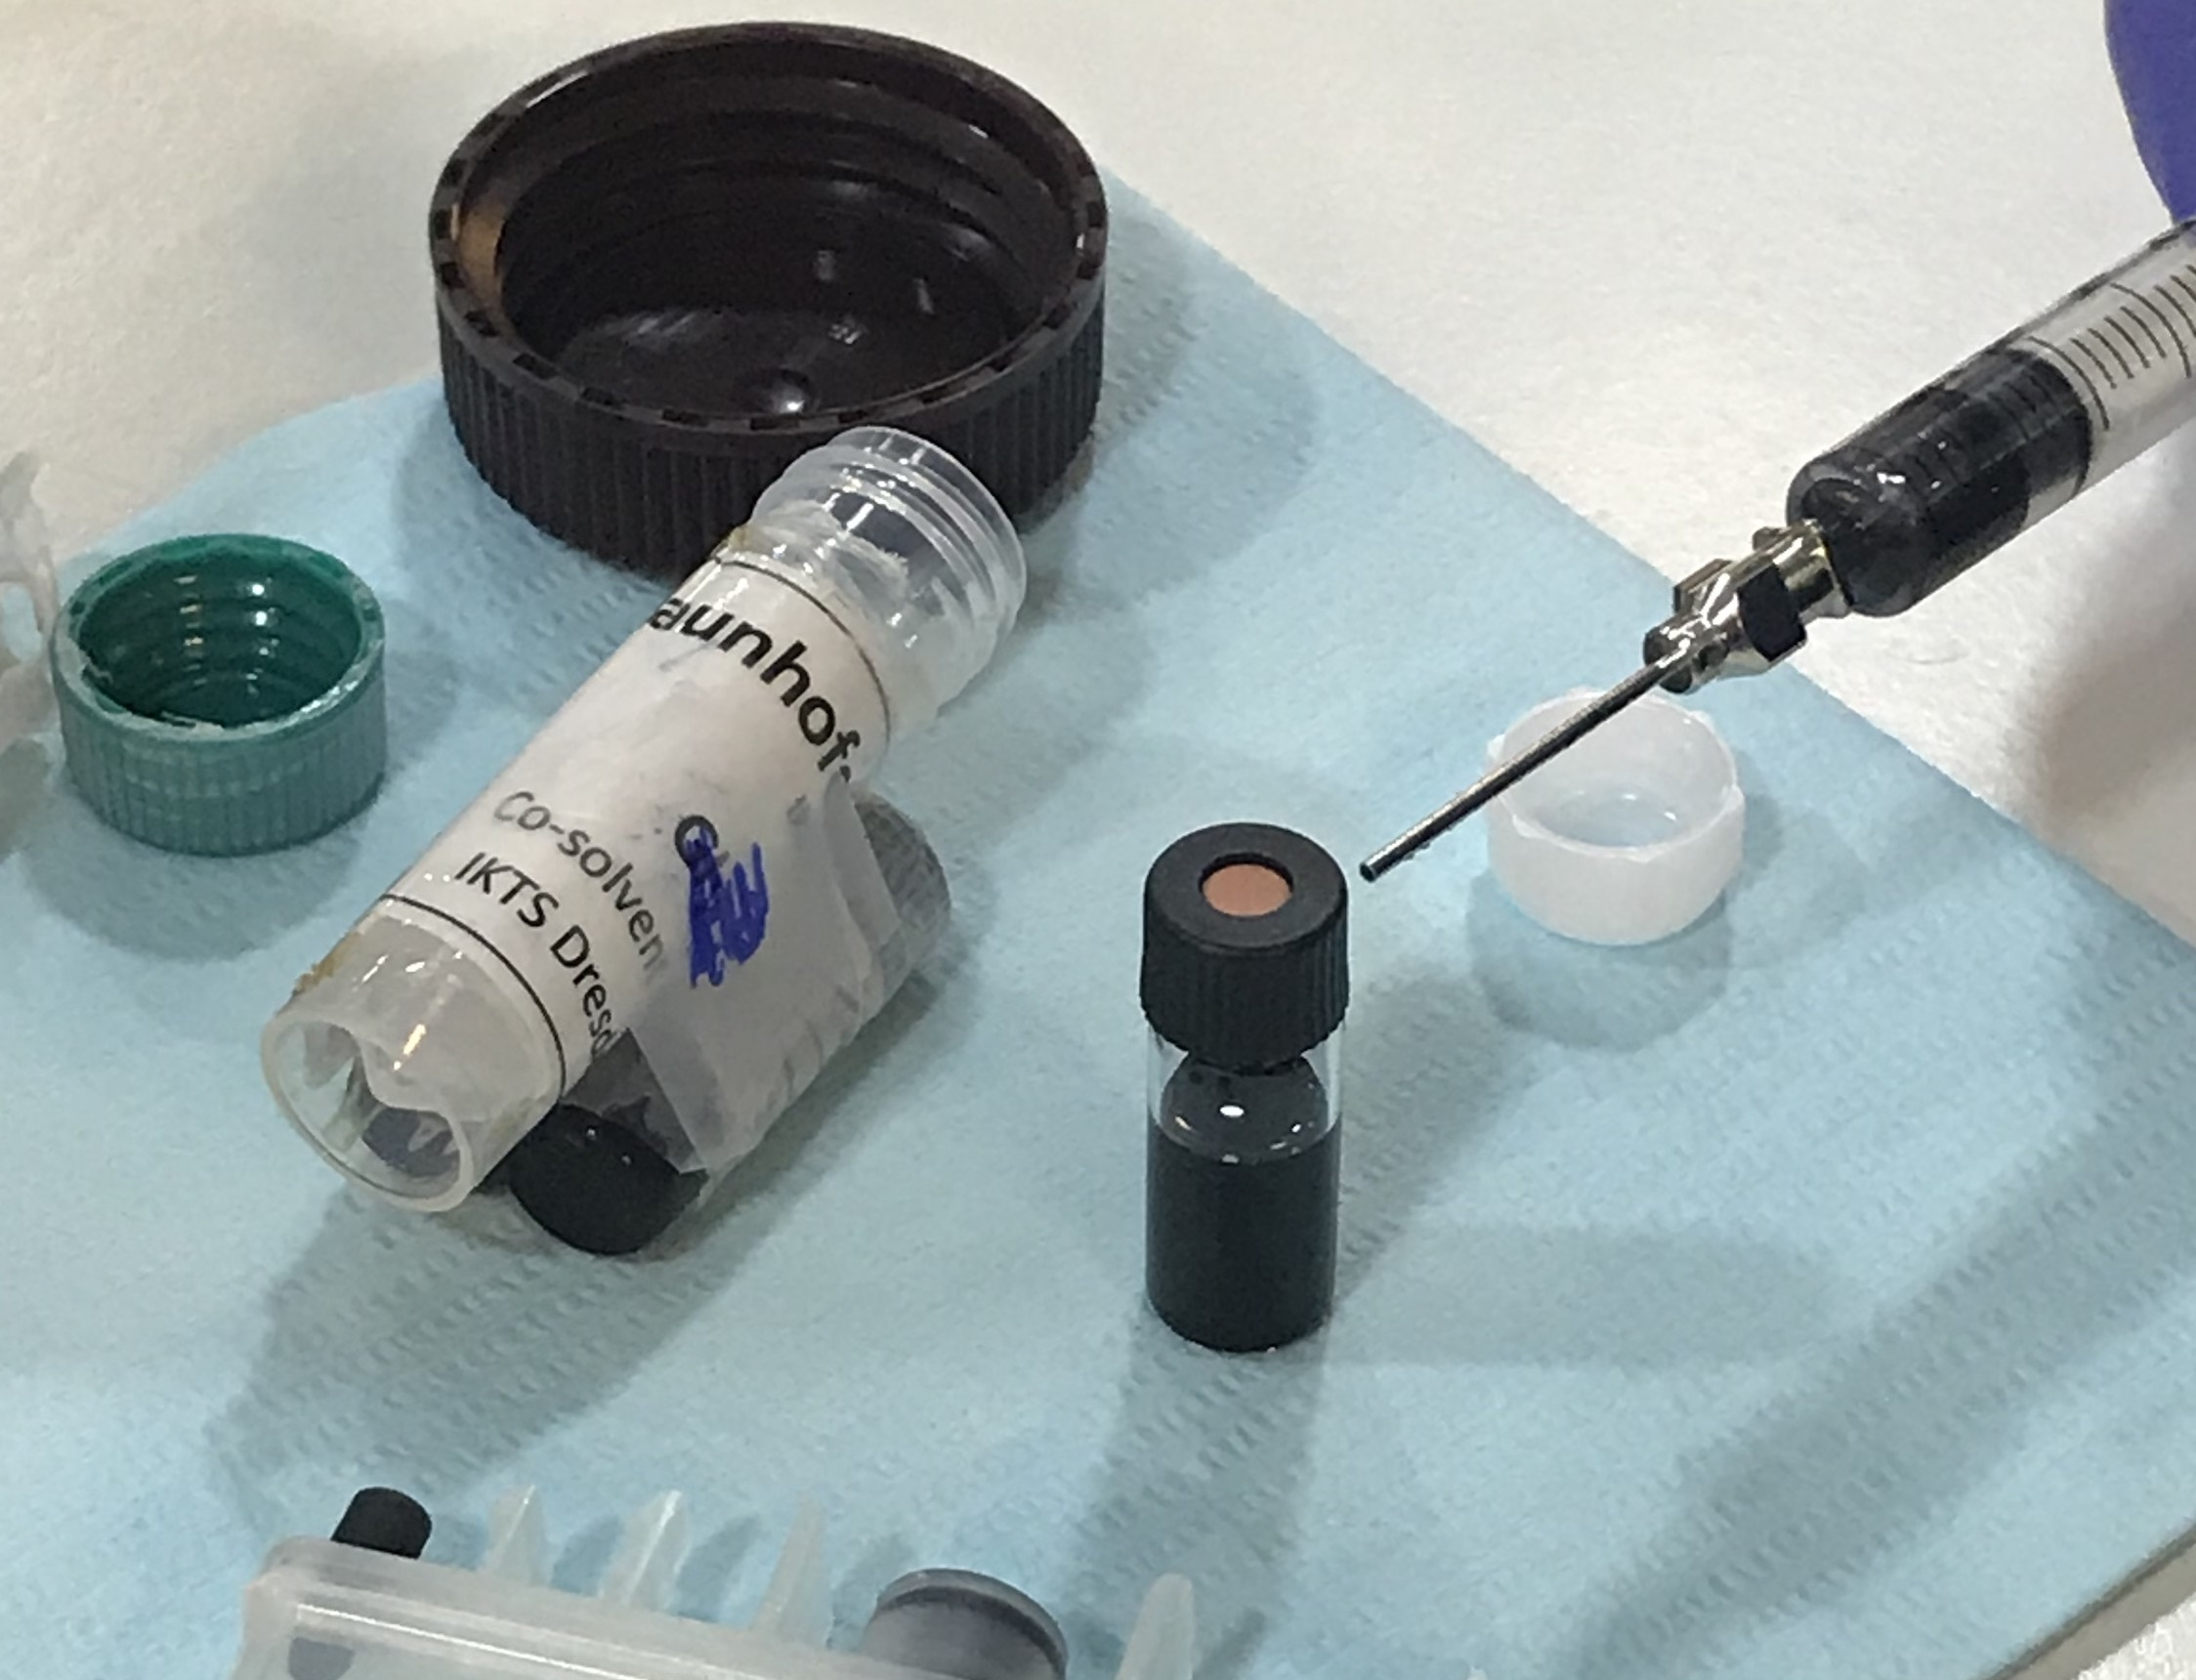
\includegraphics[width=0.5\textwidth]{Figuras/Figura_tinta_Au}
  \caption{Recipiente con tinta de nanopartículas de oro sellado herméticamente.}
  \label{fig:Figura_tinta_Au}
\end{figure}

\subsection{Tinta dieléctrica fotodefinible SU-8}
La tinta dieléctrica usada en este proyecto es \emph{PriElex SU-8 2007} de la firma \emph{MicroChem}. La misma se basa en el compuesto SU-8, es compatible con procesos de impresión por \textit{Inkjet} y puede curarse térmicamente sin la necesidad de exposición a rayos UV. (Figura ~\ref{fig:Figura_tinta_SU8}).

Algunas de sus ventajas más destacadas son su baja temperatura de curado ($<$ 150ºC), excelente estabilidad térmica y alta resistencia química.

Posee una tensión superficial de 30 dinas/cm, una densidad de 1,038 g/cm\textsuperscript{3} y una viscosidad cinemática de 9,33 cSt. Estas propiedades se encuentran informadas en la hoja de datos del fabricante \cite{PriElexSU8}.

\begin{figure}[H]
  \centering
    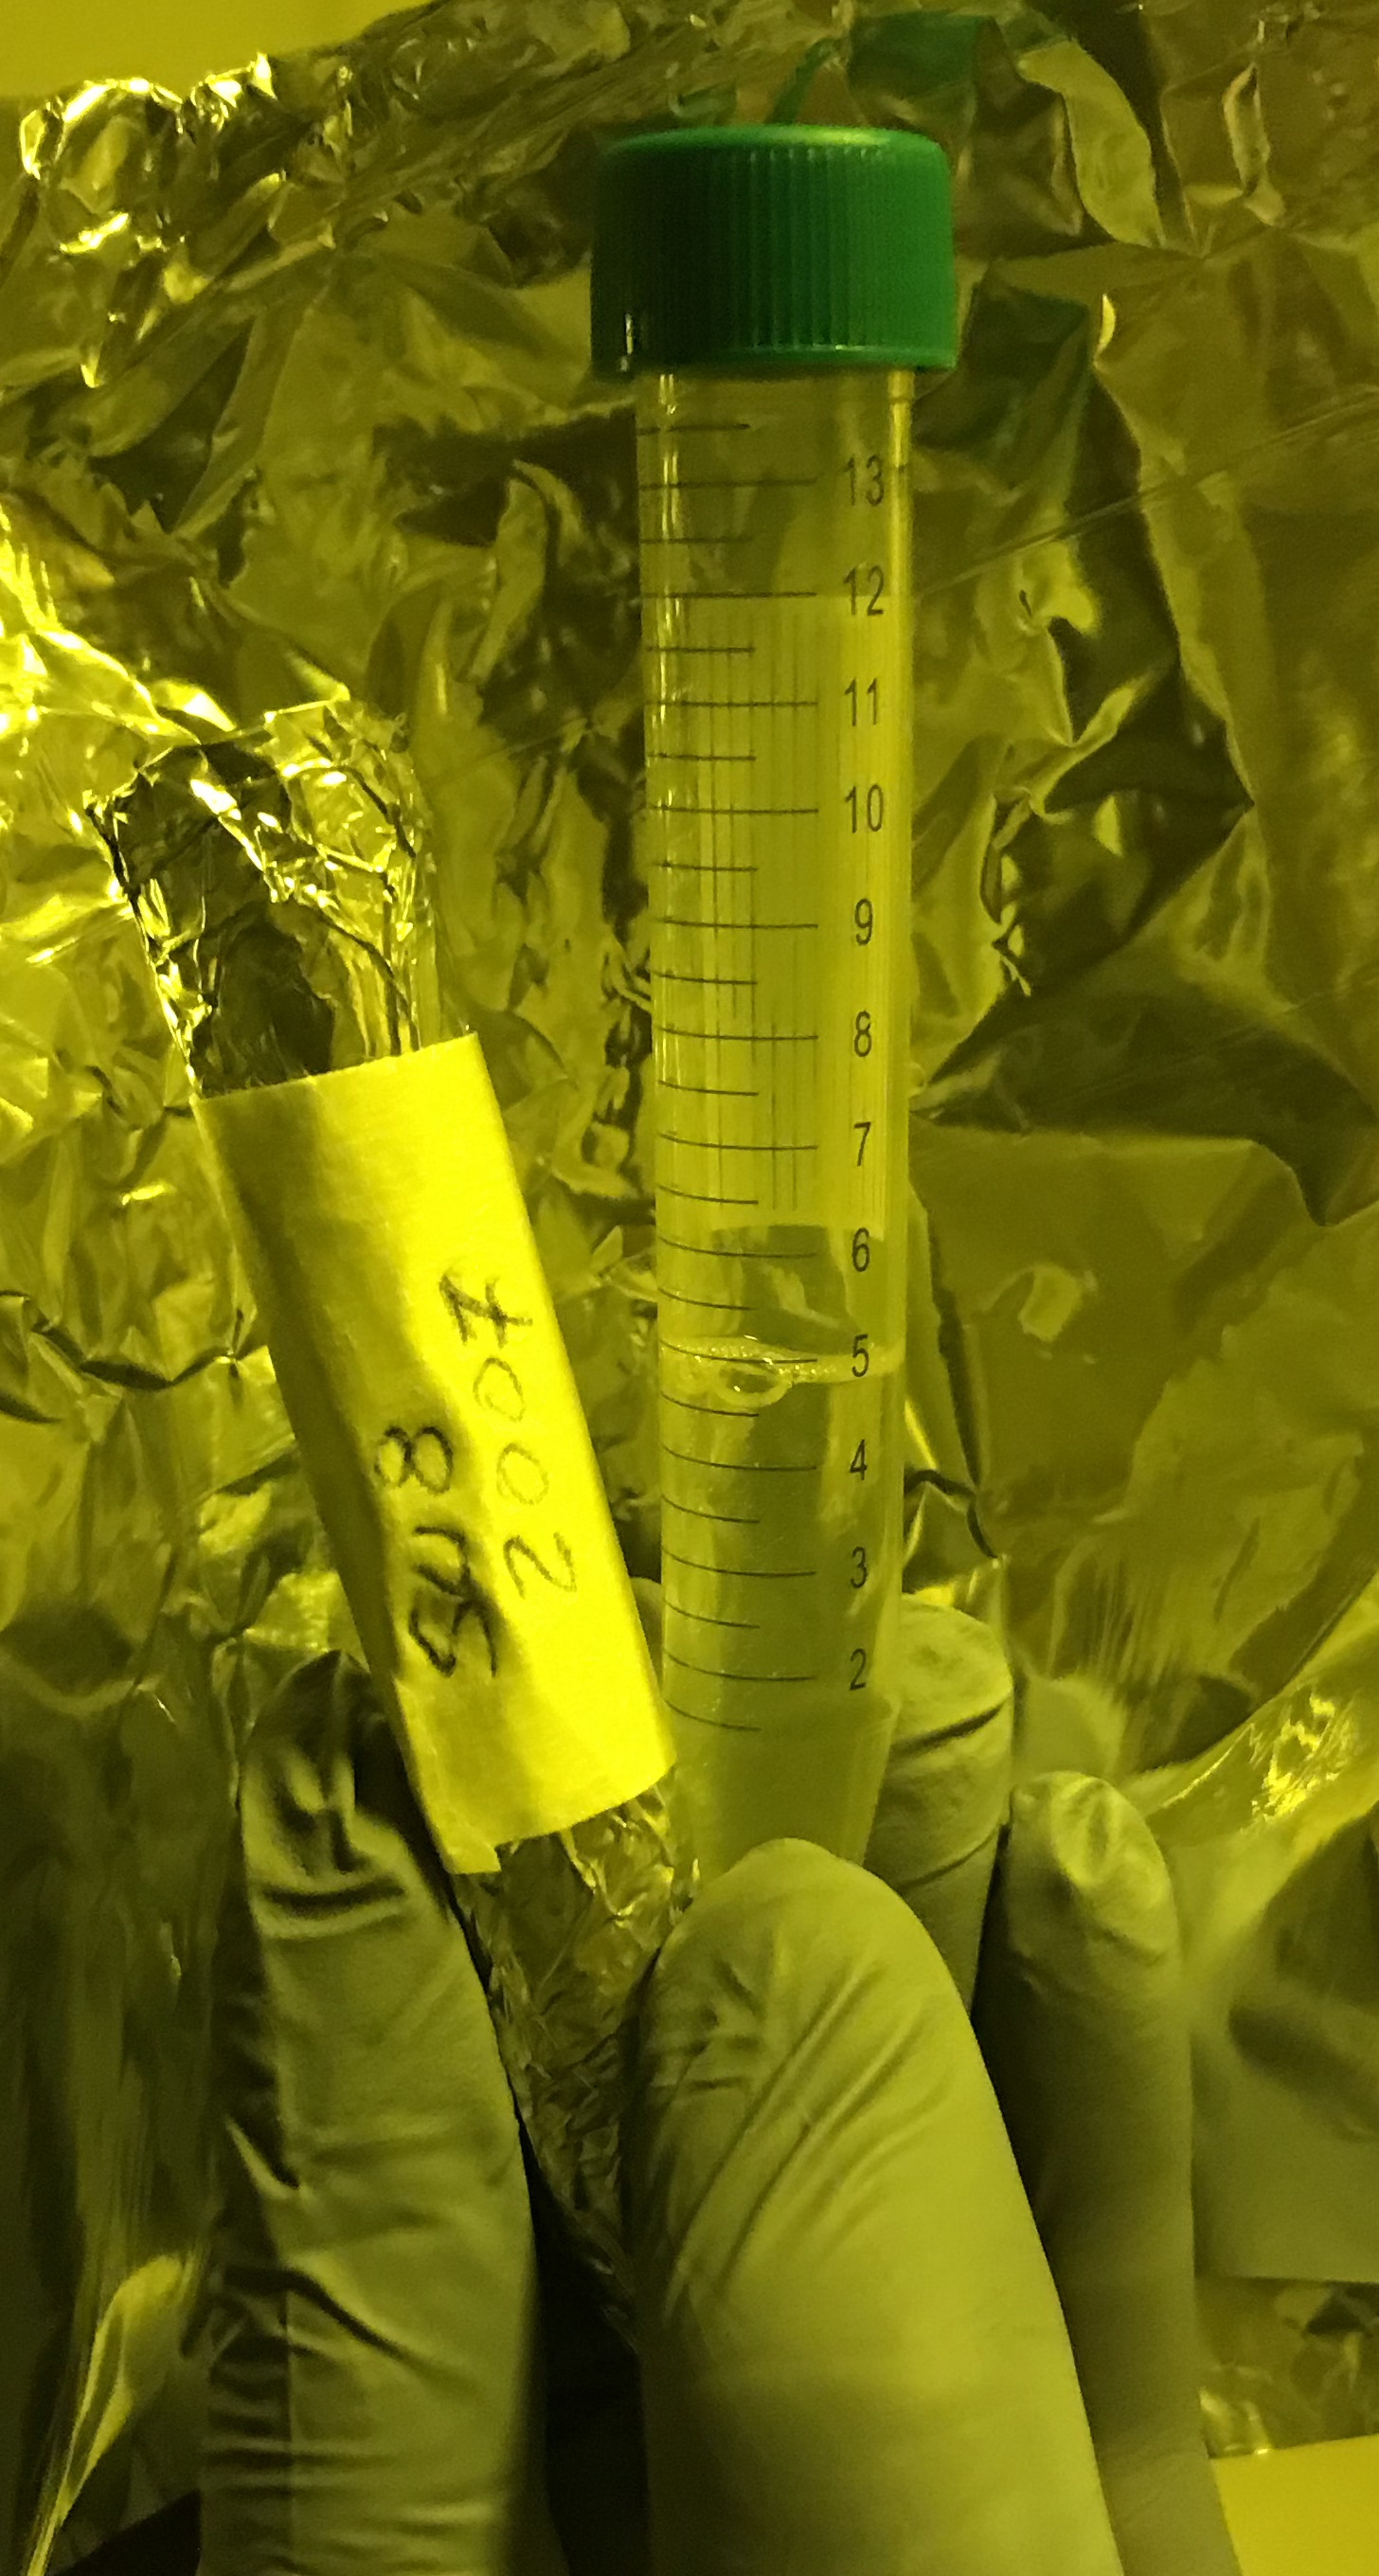
\includegraphics[width=0.2\textwidth]{Figuras/Figura_tinta_SU8}
  \caption{Recipiente con tinta dieléctrica SU-8.}
  \label{fig:Figura_tinta_SU8}
\end{figure}

\subsection{Sustrato \textit{Valox}}
El sustrato, donde se imprimirán los biosensores, es una película de tereftalita y polibutileno termoplástico. El mismo se comercializa en diferentes espesores, para este proyecto se utilizó el de 600 $\mu$m (Figura ~\ref{fig:Figura_Valox}).

Este compuesto posee una excelente resistencia dieléctrica y una fácil manipulación para realizar termoformados, estampados y doblados, lo que lo hace adecuado para una amplia gama de aplicaciones eléctricas, electrónicas y médicas \cite{Valox}.

\begin{figure}[H]
  \centering
    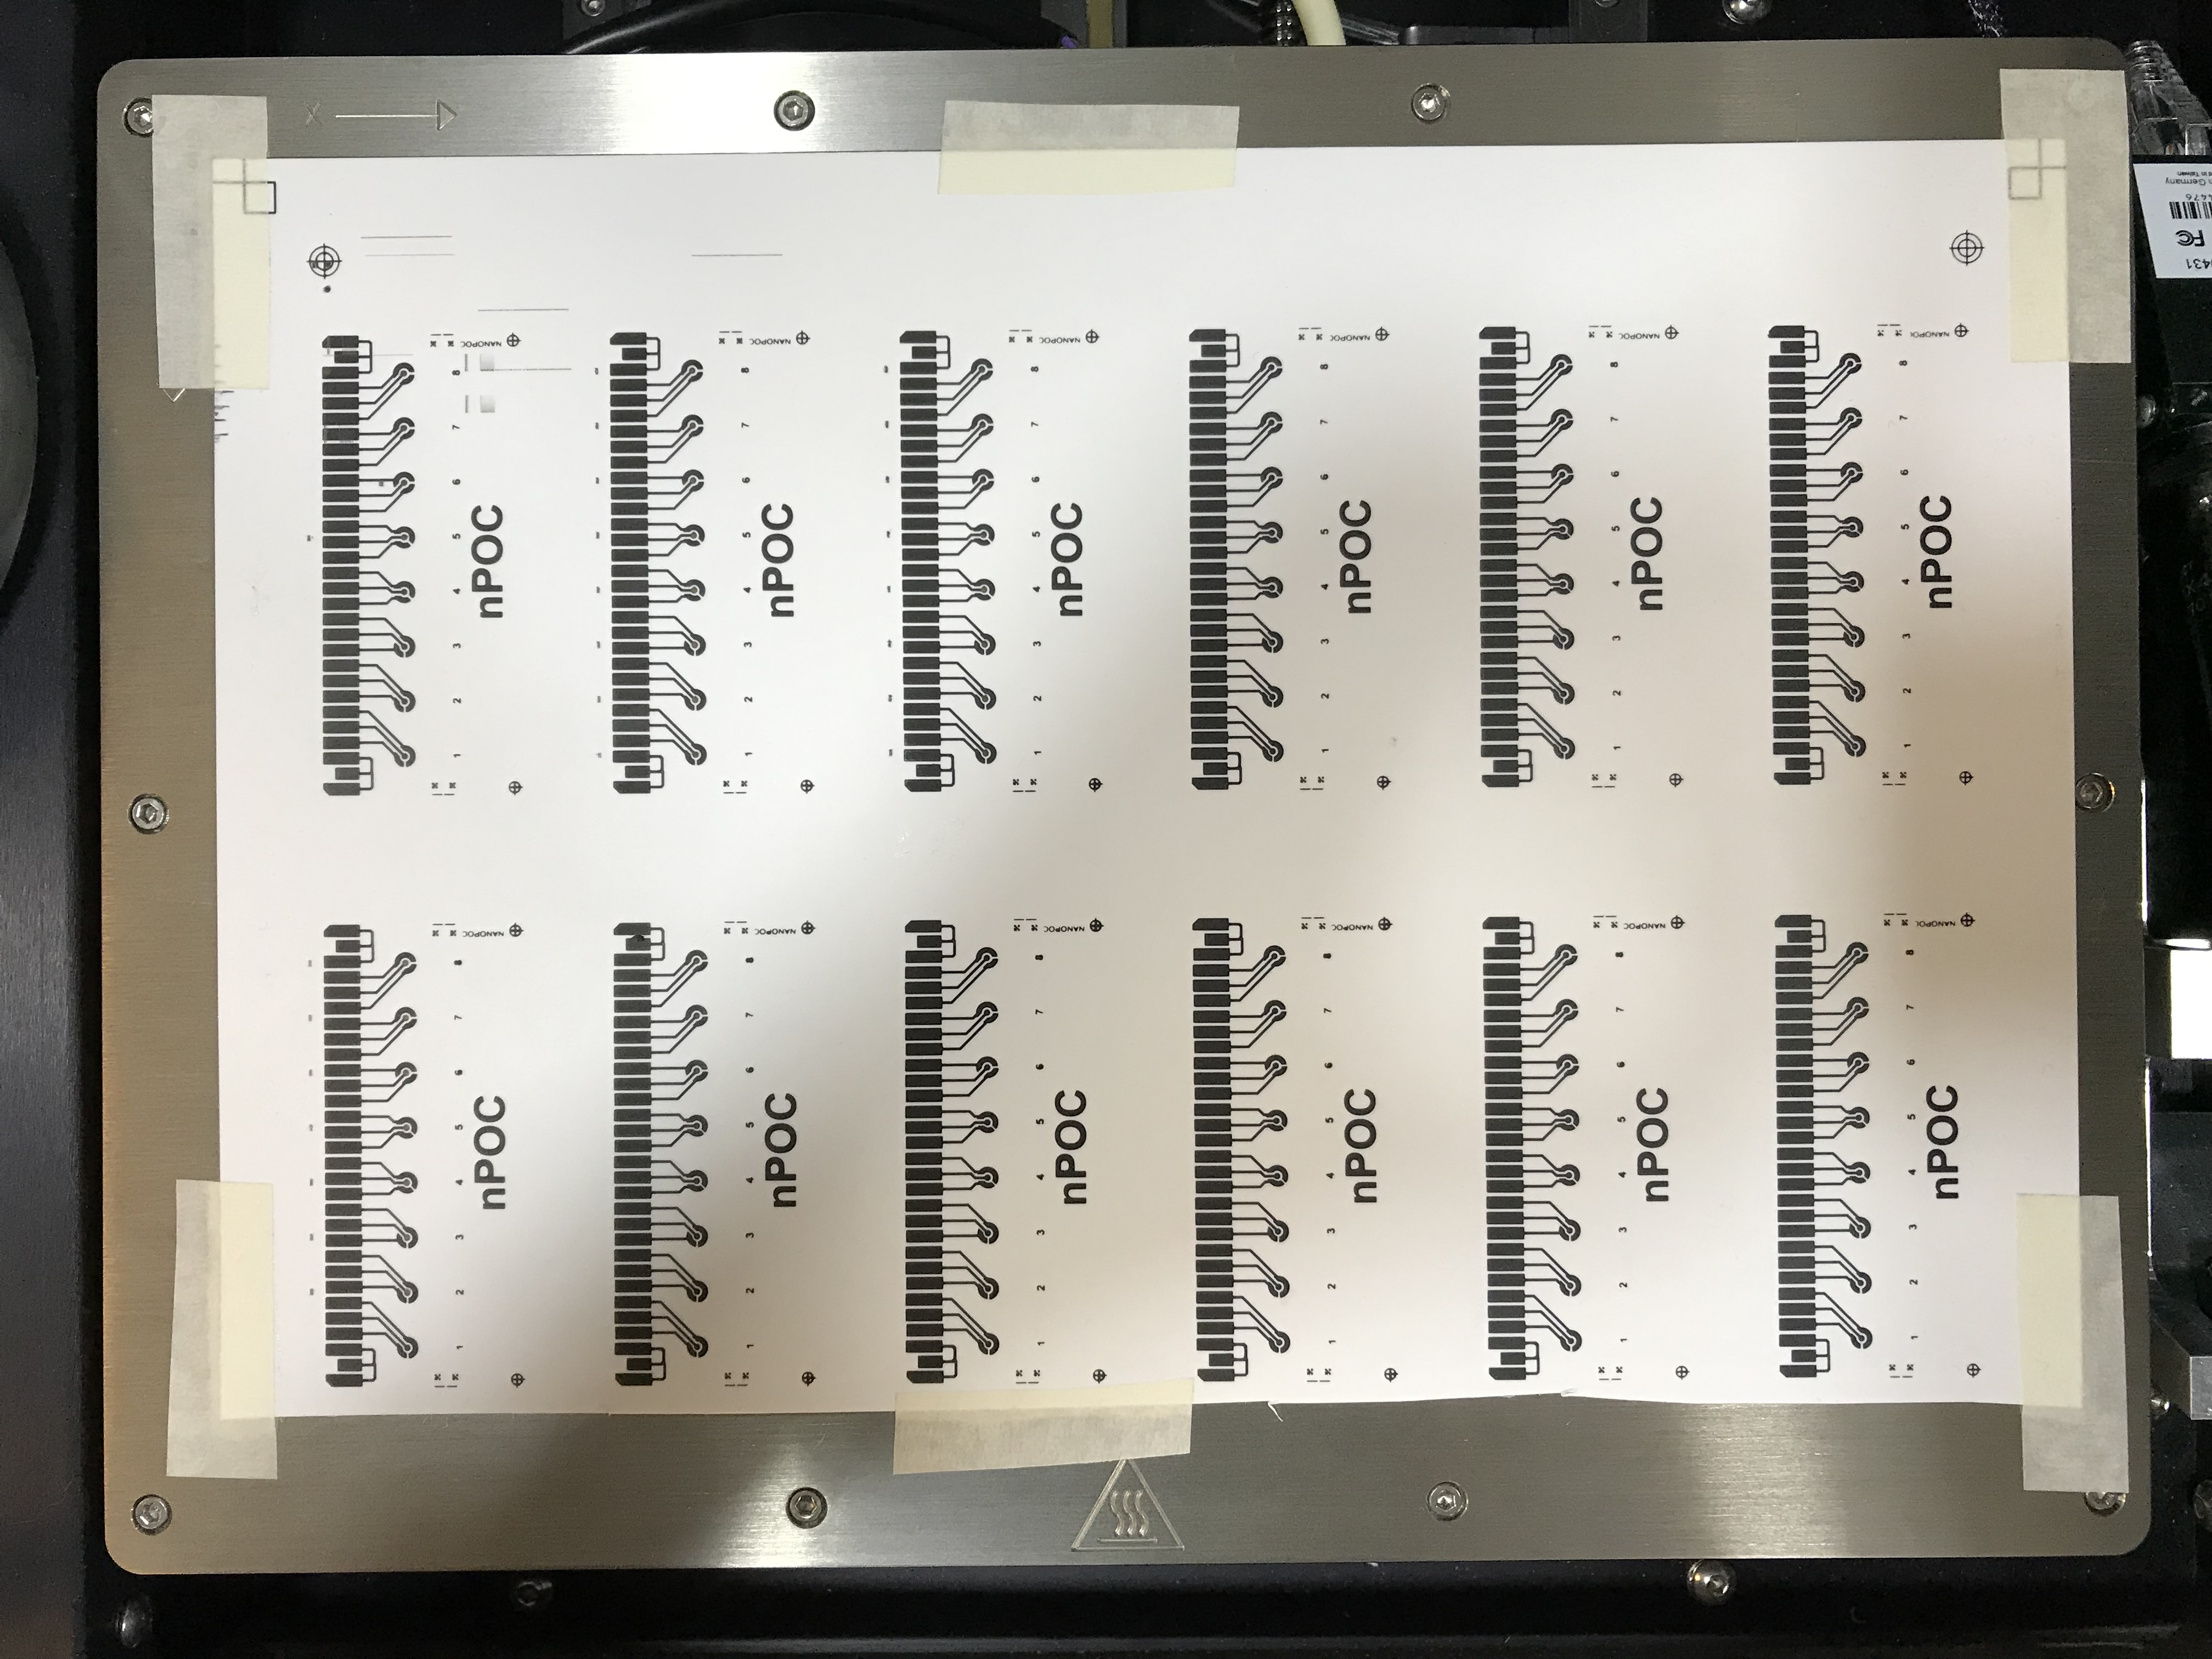
\includegraphics[width=0.55\textwidth]{Figuras/Figura_Valox}
  \caption{Sustrato \textit{Valox} con impresión serigráfica de carbono.}
  \label{fig:Figura_Valox}
\end{figure}

\section{T\'ecnicas de Caracterizaci\'on}
\subsection{Caracterizaci\'on El\'ectrica}\label{subsec:carac_elec}
Debido a la escala en que se imprime la tinta de nanopartículas puede presentar microfisuras invisibles a la vista e imágenes de poco aumento, sin embargo, son perceptibles en imágenes aumentadas por microscopio (Figura ~\ref{fig:Figura_Carac_elec}).

\begin{figure}[H]
  \centering
    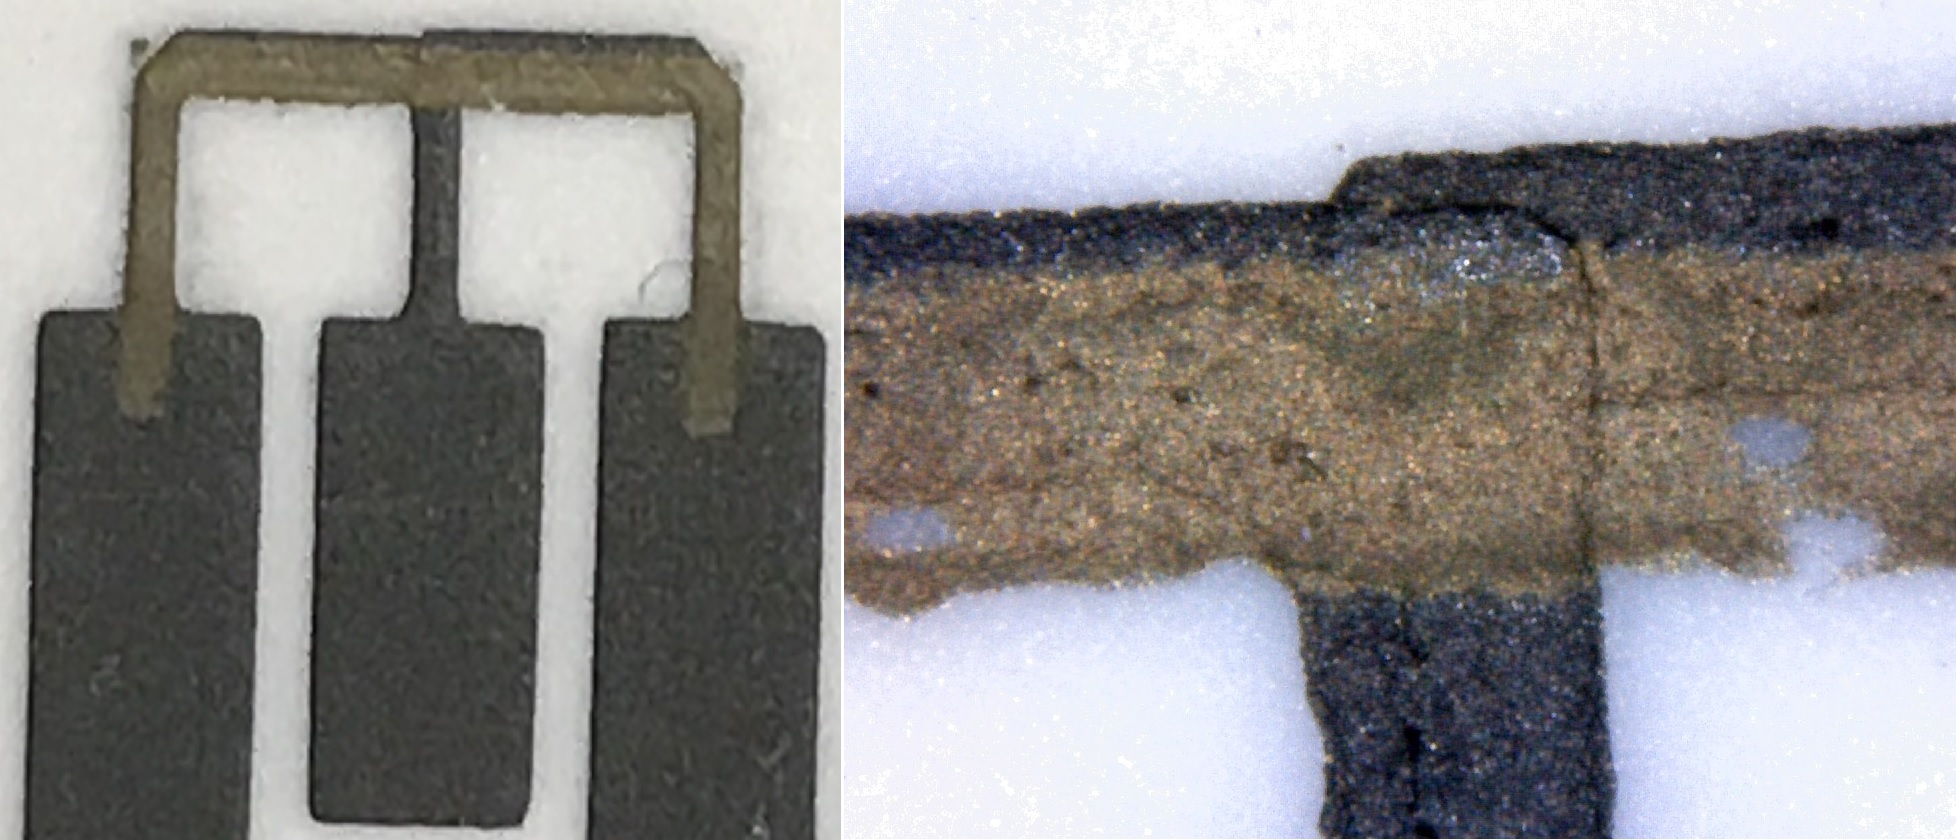
\includegraphics[width=0.5\textwidth]{Figuras/Figura_Carac_elec}
  \caption{Imagen con cámara convencional (iPhone 7) e imagen con microscopio USB Aumento 1000X.}
  \label{fig:Figura_Carac_elec}
\end{figure}

A través de una medición de resistencia a 4 puntas (conocido como método de Kelvin), se puede asegurar la continuidad física de la película, el correcto funcionamiento de la impresora y por ende del eléctrodo de trabajo del biosensor.

El método utiliza dos circuitos vinculados por una fuente de corriente continua. Por uno circula la corriente proveniente de la fuente, medida por un amperimetro y el otro posee un voltímetro en paralelo con la resistencia a medir. También se encuentra el sistema dual al anterior, dónde se tiene una fuente de tensión verificada con un voltímetro y un amperímetro que mide la corriente circulante por la resistencia (Figura ~\ref{fig:Figura_metodo_Kelvin}).

\begin{figure}[H]
  \centering
    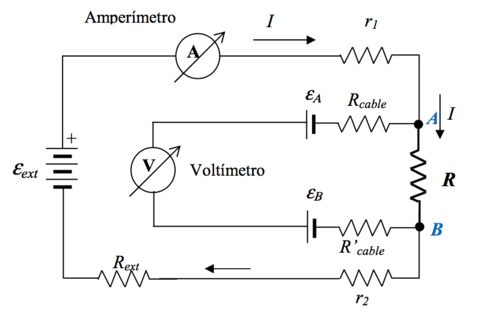
\includegraphics[width=0.5\textwidth]{Figuras/Figura_metodo_Kelvin}
  \caption{Circuito de medición a cuatro puntas.}
  \label{fig:Figura_metodo_Kelvin}
\end{figure}


\subsection{Caracterizaci\'on \'Optica/Dimensional}
Como parte de una caracterización óptica o dimensional es importante saber tamaños, espesores y rugosidades.

Los tamaños pueden obtenerse a través de la cámara fiducial de la impresora. El software de la misma permite realizar mediciones de distancias entre dos puntos y de esta forma obtener todos los valores requeridos en la caracterización (Figura ~\ref{fig:Figura_Cam_Fiducial_Medicion}).

\begin{figure}[H]
  \centering
    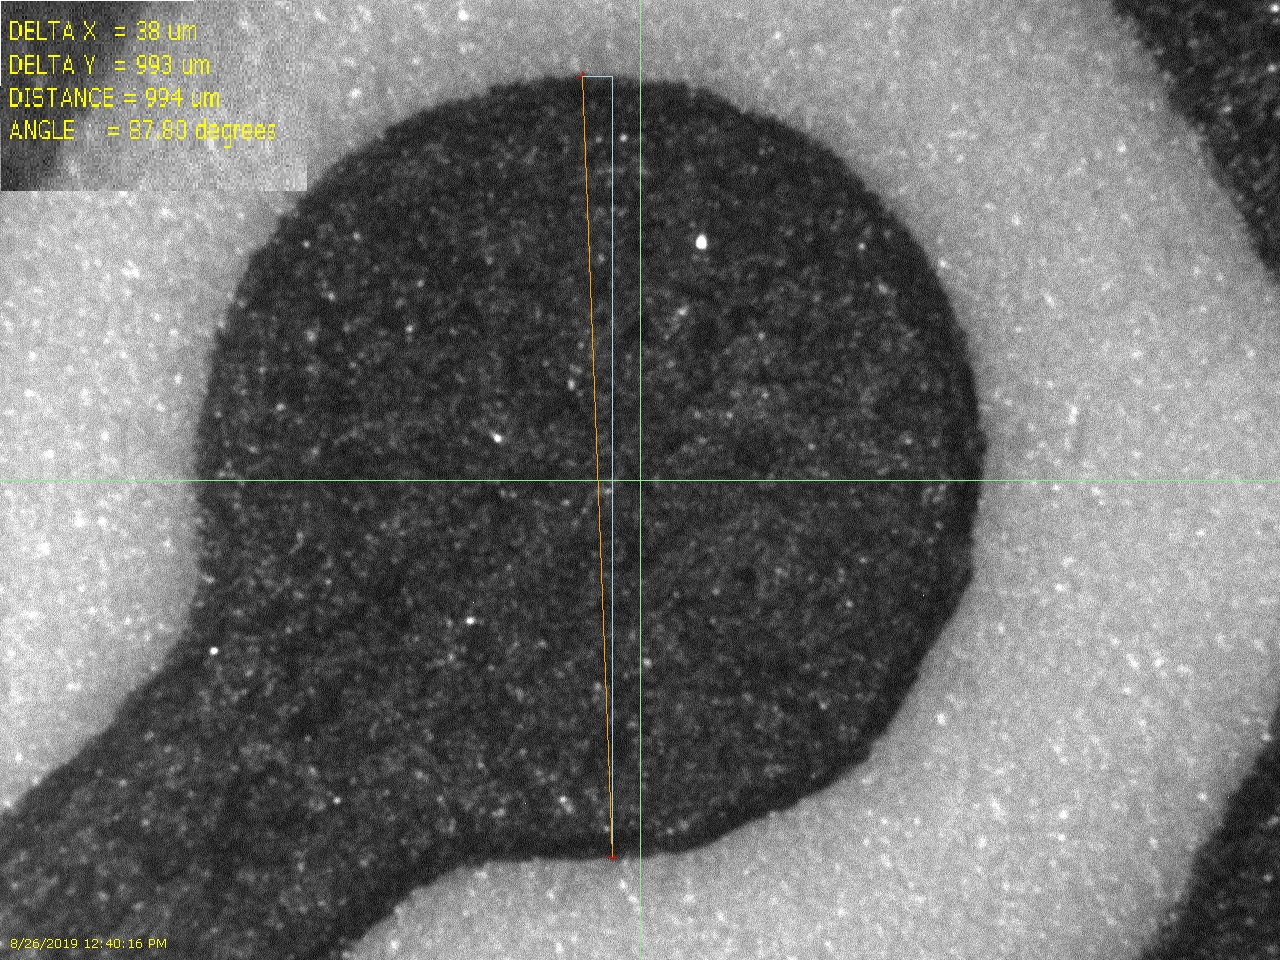
\includegraphics[width=0.5\textwidth]{Figuras/Figura_Cam_Fiducial_Medicion}
  \caption{Imagen de cámara fiducial con medición de distancias.}
  \label{fig:Figura_Cam_Fiducial_Medicion}
\end{figure}

A través de un perfilómetro de contacto se puede obtener el espesor de las impresiones y la rugosidad de las superficies. Este equipo, también llamado rugosímetro, utiliza una punta fina en contacto con la superficie a analizar (Figura ~\ref{fig:Figura_Stylus}), realizando un barrido controlado en línea recta. Las variaciones de alturas detectadas por esta punta son convertidas en señales eléctricas y pueden ser registradas o graficadas.

\begin{figure}[H]
  \centering
    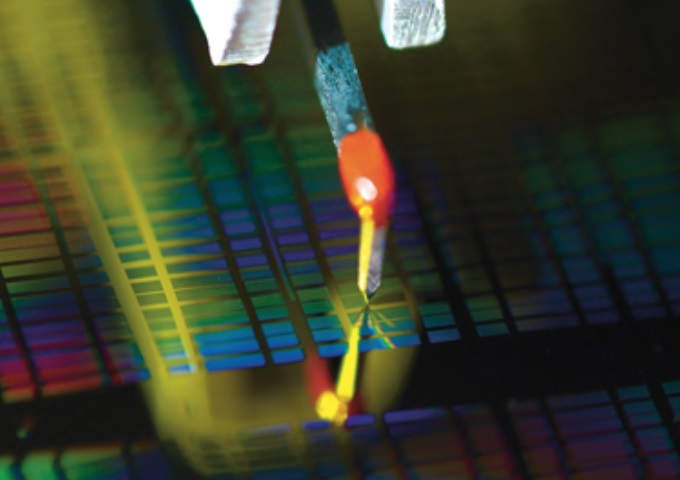
\includegraphics[width=0.5\textwidth]{Figuras/Figura_Stylus}
  \caption{Imagen de punta tipo Stylus de un perfilómetro de contacto.}
  \label{fig:Figura_Stylus}
\end{figure}

La rugosidad es un dato importante en la caracterización, ya que esta define el área efectiva de funcionamiento del biosensor. Cuanto más lisa sea la superficie, el área efectiva se aproximará al área geométrica del electrodo.

\subsection{Caracterizaci\'on Electroqu\'imica}
Para este trabajo se utiliza el procedimiento de voltametría cíclica de corriente continua. Esta caracterización electroquímica consiste en variar, de manera cíclica, el potencial del electrodo de trabajo respecto de uno de referencia. Ambos se sumergen en una solución y se mide la corriente resultante que circula por el electrodo de trabajo (Figura ~\ref{fig:Figura_circuito_voltametria}). 
\begin{figure}[H]
  \centering
    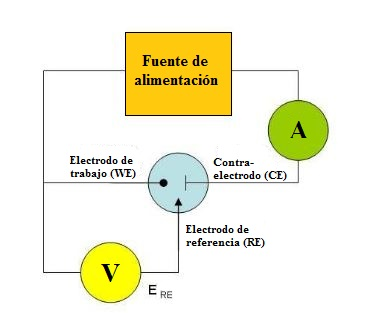
\includegraphics[width=0.65\textwidth]{Figuras/Figura_circuito_voltametria}
  \caption{Esquema de circuito eléctrico para voltametría cíclica de corriente contínua.}
  \label{fig:Figura_circuito_voltametria}
\end{figure}
La señal de excitación es un barrido de potencial lineal con una onda de forma triangular, la cual parte de un potencial E1, que evoluciona linealmente en el tiempo hasta un potencial E2 para luego volver a E1 (Figura ~\ref{fig:Figura_Carac_electroquimica}). Las velocidades de este barrido pueden variar desde menos de 1 mV/s hasta cientos de volts por segundo \cite{TesisGG}.

\begin{figure}[H]
  \centering
    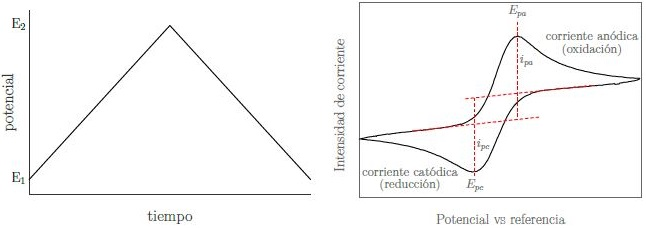
\includegraphics[width=1\textwidth]{Figuras/Figura_Carac_electroquimica}
  \caption{Curva de excitación y voltagrama típico para una especie redox reversible. Figura extraída de \cite{TesisGG}.}
  \label{fig:Figura_Carac_electroquimica}
\end{figure}

Se usaron como sondas electroquímicas ferrocianuro y ferricianuro. La elección de estas sondas se debe a la reversibilidad de los pares \textit{redox}, cuyas especies oxidada y reducida son económicas y fáciles de conseguir, solubles en solución acuosa y se comportan de forma cuasi reversible frente al intercambio electrónico.

Se espera, en la aproximación más simple, que sigan el comportamiento voltamétrico descrito por Randles-Sevcik \ref{ecuacion3}, donde la corriente pico $(i_{p})$ es proporcional a la concentración (C), a la raíz cuadrada de la velocidad de barrido (\textit{v}) y al área (A). Los demás parámetros se consideran constantes.

\begin{equation}\label{ecuacion3}
i_{p}=0,4463nFAC(\frac{nFvD}{RT})^{1/2}\
\end{equation}


